%%%%%%%%%%%%%%%%%%%%%%%%%%%%%%%%%%%%%%%%%%%%%%%%%%%%%%%%%%%%%%%%%%%%%%%%%%%%%%%
\chapter{Diagonal and Circulant Matrices for Compact Neural Networks}
\label{chapter:ch4-diagonal_circulant_neural_network}
%%%%%%%%%%%%%%%%%%%%%%%%%%%%%%%%%%%%%%%%%%%%%%%%%%%%%%%%%%%%%%%%%%%%%%%%%%%%%%%
\localtoc
% \vspace{-1cm}

% \begin{abstract}
% In this chapter, we study deep diagonal circulant neural networks, which are deep neural networks in which weight matrices are the product of diagonal and circulant ones.
% Besides making a theoretical analysis of their expressivity, we introduce principled techniques for training these models: we devise an initialization scheme and propose a smart use of nonlinearity functions in order to train deep diagonal circulant networks. 
% Furthermore, we show that these networks outperform recently introduced deep networks with other types of structured layers. We conduct a thorough experimental study to compare the performance of deep diagonal circulant networks with state-of-the-art models based on structured matrices and with dense models. We show that our models achieve better accuracy than other structured approaches while requiring 2x fewer weights than the next best approach. Finally, we train compact and accurate deep diagonal circulant networks on a real world video classification dataset with over 3.8 million training examples. 
% \end{abstract}

%%%%%%%%%%%%%%%%%%%%%%%%%%%%%%%%%%%%%%%%%%%%%%%%%%%%%%%%%%%%%%%%%%%%%%%%%%%%%%%%
\section{Introduction}
\label{chapter:ch4-introduction}
%%%%%%%%%%%%%%%%%%%%%%%%%%%%%%%%%%%%%%%%%%%%%%%%%%%%%%%%%%%%%%%%%%%%%%%%%%%%%%%%


In recent years, designing compact and accurate neural networks with a small number of trainable parameters has been an active research topic.
It is motivated by practical applications in embedded systems (to reduce memory footprint \cite{sainath2015convolutional}), federated and distributed learning (to reduce communication \cite{konecny2016federated}), etc.
% derivative-free optimization in reinforcement learning (to simplify the computation of the approximated gradient \cite{choromanski2018structured}), etc.
Besides a number of practical applications, it is also an important research question whether or not models really need to be this large or if smaller networks can achieve similar accuracy~\cite{ba2014deep}.

Structured matrices are at the very core of most of the work on compact networks.
In these models, dense weight matrices are replaced by matrices with a prescribed structure (\eg, low rank matrices, Toeplitz matrices, circulant matrices, LDR, etc.).
Despite substantial efforts  (\eg, \citet{cheng2015exploration,moczulski2016acdc}), the performance of compact models is still far from achieving an acceptable accuracy motivating their use in real-world scenarios.
This raises several questions about the effectiveness of such models and about our ability to train them.
In particular two main questions call for investigation:
% \begin{enumerate}[parsep=0pt,topsep=0pt]
% \begin{enumerate}[itemsep=0pt,leftmargin=0pt]
\begin{enumerate}
    \item \emph{What is the expressive power of structured layers compared to dense layers?}
    % \item \emph{What is the expressive power of diagonal-circulant neural networks compared to dense ones?}
    \item \emph{How to efficiently train deep neural networks with a large number of structured layers?}
    % \item \emph{How to efficiently train diagonal-circulant neural networks with a large number of layers?}
    % \item \emph{How to efficiently train diagonal-circulant neural networks with a large depth?}
\end{enumerate}
In this chapter we aim at answering these questions by studying deep diagonal-circulant neural networks (\aka DCNNs), which are deep neural networks in which weight matrices are the product of diagonal and circulant ones.
The idea of using diagonal and circulant matrices together comes from a series of results in linear algebra by~\citet{muller1998algorithmic} and~\citet{huhtanen2015factoring}.
% The most recent result from~\cite{huhtanen2015factoring} demonstrates that any matrix can be decomposed into the product of $2n-1$ alternating diagonal and circulant matrices.

To answer the first question, we propose an analysis of the expressivity of DCNNs by extending the results obtained by~\citet{huhtanen2015factoring} which states that any matrix can be decomposed into the product of $2n-1$ alternating diagonal and circulant matrices.
We introduce a new bound on the number of diagonal-circulant products required to approximate a matrix that depends on its rank.
Building on this result, we demonstrate that a DCNN with bounded width and small depth can approximate any dense neural networks with ReLU activations. 

To answer the second question, we first describe a theoretically sound initialization procedure for DCNN which allows the signal to propagate through the network without vanishing or exploding.
Furthermore, we provide a number of empirical insights to explain the behavior of DCNNs and show the impact of the number of the nonlinearities in the network on the convergence rate and the accuracy of the network. 
By combining all these insights, we are able (for the first time) to train large and deep DCNNs and demonstrate the good performance of these networks on a large-scale application (the \yt video classification problem) and obtain very competitive accuracy. 

The chapter is organized as follows:
\Cref{section:ch4-diagonal_and_circulant_matrices_for_matrix_decomposition} introduces our new result extending the one from \citet{huhtanen2015factoring}.
\Cref{section:ch4-analysis_of_diagonal_circulant_neural_networks} proposes a theoretical analysis on the expressivity of DCNNs.
\Cref{section:ch4-how_to_train_deep_diagonal_circulant_neural_networks} describes two efficient techniques for training deep diagonal circulant neural networks.
\Cref{section:ch4-experiments} presents extensive experiments to compare the performance of deep diagonal circulant neural networks in different settings with respect to other state-of-the-art approaches.
Finally, \Cref{section:ch4-discussion} provides concluding remarks. 




%%%%%%%%%%%%%%%%%%%%%%%%%%%%%%%%%%%%%%%%%%%%%%%%%%%%%%%%%%%%%%%%%%%%%%%%%%%%%%%
% \section{A Primer on the Expressivity of Circulant Matrices and a New Result}
% \label{section:ch4-a_primer_on_circulant_matrices_and_a_new_result}
\section{Diagonal and Circulant Matrices for Matrix Decomposition}
\label{section:ch4-diagonal_and_circulant_matrices_for_matrix_decomposition}
%%%%%%%%%%%%%%%%%%%%%%%%%%%%%%%%%%%%%%%%%%%%%%%%%%%%%%%%%%%%%%%%%%%%%%%%%%%%%%%

As seen in the Related Work (\Cref{chapter:ch3-related_work}), circulant matrices exhibit several interesting properties from the perspective of numerical computations.
Most importantly, any $n \times n$ circulant matrix $\Cmat$ can be represented using only $n$ coefficients instead of the $n^2$ coefficients required to represent classical unstructured matrices.
In addition, the matrix-vector product is simplified from $\bigO(n^2)$ to $\bigO(n \log n)$ using the  convolution theorem.
As we will show in this chapter, circulant matrices also have a strong expressive power.
So far, we know that a single circulant matrix can be used to represent a variety of important linear transforms such as random projections~\cite{hinrichs2011johnson}. 
However, when they are combined with diagonal matrices, they can also be used as building blocks to represent any linear transform~\cite{schmid2000decomposing,huhtanen2015factoring} with an arbitrary precision.

First, we are interested in the relation between the product of diagonal and circulant matrices and low-rank matrices.
\citet{huhtanen2015factoring} were able to bound the number of factors that is required to approximate any matrix $\Amat$ with arbitrary precision.
We recall this result in \Cref{theorem:ch4-huhtanen} as it is the starting point of our theoretical analysis.

\begin{theorem}[Reformulation from \citet{huhtanen2015factoring}] \label{theorem:ch4-huhtanen}
  For every matrix $\Mmat \in \Cnn$, for any $\epsilon > 0$, there exists a sequence of matrices $\Amat^{(1)} \ldots \Amat^{(2n-1)}$ where $\Amat^{(i)}$ is a circulant matrix if $i$ is odd, and a diagonal matrix otherwise, such that
  \begin{equation}
    \norm{\Amat^{(1)} \ldots \Amat^{(2n-1)} - \Mmat}_\fro < \epsilon \enspace.
  \end{equation}
  \removespace
\end{theorem}

This result has an elegant interpretation in the context of \emph{optical image processing}.
Indeed, this result can be seen as the signal being scaled alternatively in the original domain and in the Fourier domain by using the decomposition of circulant matrices with the Fourier matrix (see \Cref{theorem:ch2-diagonalization_circulant_matrix}):
\begin{equation}
  \norm{ \frac{1}{n^{(n-1)}} \left( \Umat_n^* \Dmat^{(1)} \Umat_n \Dmat^{(2)} \dots \Umat_n^* \Dmat^{(2n-1)} \Umat_n \right) - \Mmat}_\fro \leq \epsilon \enspace,
\end{equation}
where each matrix $\Dmat^{(i)} \in \Cbb^{n \times n}$ is a diagonal.
Because any unitary matrix can be interpreted as being a diffractive optical system, this decomposition can be `implemented' using a cascade of lenses \cite{muller1998algorithmic}.


% In particular, any unitary matrix A ∈ Cn×n can be interpreted as being a diffractive optical
% system. See [15] how products of discrete Fourier transforms and diagonal matrices model diffractive
% optical elements.

% This result has been demonstrated in the context of \emph{optical image processing} where  

% The signal is scaled alternatively in the original domain and in the Fourier domain. 

% Or, alternatively, purely Fourier analytically one can view this as a factorization involving discrete
% Fourier transforms and diagonal matrices.3

% There exists an elegant result, motivated by applications in optical image processing, stating that any matrix A ∈ C
% n×n is the product of circulant and diagonal matrices [15, 18].1

% \citet{hermans2015towards}
% => In a separate research community, Hermans & Vaerenbergh (2015) recently discussed using waves
% in a trainable medium for learning linear layers by backpropagation, and suggested a potential implementation using an integrated photonics chip. The nanophotonic chip consists of a cascade of
% unitary trasformations of the optical signals interleaved with tuneable waveguides (phase shifters).
% Hermans & Vaerenbergh (2015) present an abstraction of this chip. I


% \todotext{dire pourquoi ce theorem est interessant, expliquer le relation avec optic et Fourier et continuer avec les limites du théoèrme}
% \todotext{faire le lien avec le background et les travaux de ACDC}

Unfortunately, this theorem is of little use to understand the expressive power of diagonal-circulant matrices when they are used in deep neural networks for two reasons:
\begin{enumerate}%[parsep=0pt,itemsep=0pt,topsep=0pt]
  \item the bound only depends on the dimension of the matrix $\Mmat$, not on the matrix itself;
  \item the theorem does not provide any insights regarding the expressive power of $m$ diagonal-circulant factors when $m$ is much lower than $2n - 1$ as it is the case in most practical scenarios we consider in this chapter. 
\end{enumerate}

In the following theorem, we enhance the result of~\citet{huhtanen2015factoring} by expressing the number of factors required to approximate $\Mmat$, \emph{as a function of the rank of $\Mmat$}.
This is useful when one deals with low-rank matrices, which is common in machine learning problems. 
\begin{maintheorem}[Rank-based diagonal-circulant decomposition] \label{theorem:ch4-rank-decomposition}
  Let $\Amat \in \Cnn$ be a matrix of rank at most $k$.
  Assume that $n$ can be divided by $k$.
  For any $\epsilon > 0$, there exists a sequence of $4k+1$ matrices $\Amat^{(1)} \ldots \Amat^{(4k+1)}$, where $\Amat^{(i)}$ is a circulant matrix if $i$ is odd, and a diagonal matrix otherwise, such that $\norm{\Amat^{(1)} \ldots \Amat^{(4k+1)} - \Mmat} < \epsilon$.
\end{maintheorem}

\begin{proof}[\Cref{theorem:ch4-rank-decomposition}]
Let $\Umat \mathbf{\Sigma} \Vmat^\top$ be the SVD decomposition of $\Mmat$ where $\Umat,\Vmat$ and $\mathbf{\Sigma}$ are $n \times n$ matrices.
Because $\Mmat$ is of rank $k$, the last $n-k$ columns of $\Umat$ and $\Vmat$ are null.
In the following, we will first decompose $\Umat$ into a product of matrices $\Wmat\Rmat\Omat$, where $\Rmat$ and $\Omat$ are respectively circulant and diagonal matrices, and $\Wmat$ is a matrix which will be further decomposed into a product of diagonal and circulant matrices.
Then, we will apply the same decomposition technique to $\Vmat$.
Ultimately, we will get a product of $4k+1$ matrices alternatively diagonal and circulant.

Let $\Rmat = \circulant(r_{0}\ldots r_{n-1})$. Let $\Omat$ be a $n \times n$ diagonal matrix where $\leftmat \Omat \rightmat_{i,i} = 1$ if $i \le k$ and $0$ otherwise.
The $k$ first columns of the product $\Rmat\Omat$ will be equal to that of $\Rmat$, and the $n-k$ last columns of $\Rmat\Omat$ will be zeros. For example, if $k=2$, we have: 

\begin{equation}
  \Rmat\Omat = \leftmatrix
  r_{0} & r_{n} & 0 & \cdots & 0\\
  r_{1} & r_{0}\\
  r_{2} & r_{1} & \vdots &  & \vdots\\
  \vdots & \vdots\\
  r_{n} & r_{n-1} & 0 & \cdots & 0
  \rightmatrix
\end{equation}

\noindent
Let us define $k$ diagonal matrices $\Dmat^{(i)} = \diagonal(d_1^{(i)} \ldots d_n^{(i)})$ for $i \in [k]$.
For now, the values of $d_{j}^{(i)}$ are unknown, but we will show how to compute them.
Let $\Wmat = \sum_{i=1}^{k} \Dmat^{(i)} \Zmat_1^{i-1}$ where $\Zmat_1$ is a $1$-unit-circulant matrix defined in \Cref{chapter:ch2-background},~\Cref{subsection:ch2-toeplitz_and_circulant_matrices}.
Note that the $n-k$ last columns of the product $\Wmat\Rmat\Omat$ will be zeros.
For example, with $k=2$, we have: 

\begin{equation}
  \Wmat = \leftmatrix
  d_{1}^{(1)} &  &  &  & d_{1}^{(2)} \\
  d_{2}^{(2)} & d_{2}^{(1)} \\
   & d_{3}^{(2)} & \ddots \\
   &  & \ddots & \ddots \\
   &  &  & d_{n}^{(2)} & d_{n}^{(1)}
  \rightmatrix
\end{equation}

\begin{equation}
  \Wmat\Rmat\Omat = \leftmatrix
  r_{1} d_{1}^{(1)} + r_{n}   d_{1}^{(2)} & r_{n}   d_{1}^{(1)} + r_{n-1} d_{1}^{(2)} & 0 & \cdots & 0 \\
  r_{2} d_{2}^{(1)} + r_{1}   d_{2}^{(2)} & r_{1}   d_{2}^{(1)} + r_{n}   d_{2}^{(2)} & 0 & \cdots & 0 \\
  \vdots & \vdots & \vdots &  & \vdots \\
  r_{n} d_{n}^{(1)} + r_{n-1} d_{n}^{(2)} & r_{n-1} d_{n}^{(1)} + r_{n-2} d_{n}^{(2)} & 0 & \cdots & 0
  \rightmatrix
\end{equation}

% TODO: revoir ce passage, un peu complexe
\noindent
We want to find the values of $d_{j}^{(i)}$ such that $\Wmat \Rmat \Omat = \Umat$.
We can formulate this as linear equation system.
In case $k=2$, we get:

\begin{equation}
  \leftmatrix
  r_{n} & r_{1}\\
  r_{n-1} & r_{n}\\
   &  & r_{1} & r_{2}\\
   &  & r_{n} & r_{1}\\
   &  &  &  & r_{2} & r_{3}\\
   &  &  &  & r_{1} & r_{2}\\
   &  &  &  &  &  & \ddots\\
   &  &  &  &  &  &  & \ddots
  \rightmatrix \times \leftmatrix
  d_{1}^{(2)} \\
  d_{1}^{(1)} \\
  d_{2}^{(2)} \\
  d_{2}^{(1)} \\
  d_{3}^{(2)} \\
  d_{3}^{(1)} \\
  \vdots\\
  \vdots
  \rightmatrix = \leftmatrix
  (\Umat)_{0,0} \\
  (\Umat)_{0,1} \\
  (\Umat)_{1,0} \\
  (\Umat)_{1,1} \\
  \\
  \\
  \vdots\\
  \\
  \rightmatrix
\end{equation}

\noindent
The $i^{th}$ block of the block-diagonal matrix is a Toeplitz matrix induced by a subsequence of length $k$ of $(r_1,\ldots r_n,r_1 \ldots r_n)$.
Set $r_{j}=1$ for all $j\in\{k,2k,3k,\ldots n\}$ and set $r_{j}=0$ for all other values of $j$.
Then it is easy to see that each block is a permutation of the identity matrix.
Thus, all blocks are invertible.
This entails that the block diagonal matrix above is also invertible.
So by solving this set of linear equations, we find $d_{1}^{(1)} \ldots d_{n}^{(k)}$ such that $\Wmat\Rmat\Omat=\Umat$.
We can apply the same idea to factorize $\Vmat = \Wmat' \Rmat \Omat$ for some matrix $\Wmat'$.
Finally, we get 
\begin{equation}
  \Amat = \Umat \mathbf{\Sigma} \Vmat^\top = \Wmat\Rmat\Omat \mathbf{\Sigma} \Omat^\top \Rmat^\top \Wmat^{'\top}
\end{equation}

\noindent
Note that the matrix $\Wmat\Rmat$ can be decomposed as follows:
\begin{equation}
  \Wmat\Rmat = \left( \sum_{i=0}^{k-1} \Dmat^{(i)} \Zmat_1^{(i-1)} \right) + \Dmat^{(k)} \Zmat_1^{(k-1)} \Rmat
\end{equation}
where the last matrix $\Zmat_1^{(k-1)} \Rmat$ is a circulant matrix because both matrices are circulant (see \Cref{theorem:ch2-diagonalization_circulant_matrix}).
The same reasoning can be applied with the matrix $\Rmat^\top\Wmat'^\top$.
Therefore, by construction, the matrices $\Wmat\Rmat$ and $\Rmat^\top\Wmat'^\top$ can both be factor by $2k$ circulant and diagonal matrices.
Also note that $\Omat \mathbf{\Sigma} \Omat^\top$ is a diagonal matrix, because all three are diagonal.
Overall, $\Amat$ can be represented with a product of $4k+1$ matrices, alternatively diagonal and circulant.
\end{proof}

% TODO: ici on peut developper un peu plus
A direct consequence of \Cref{theorem:ch4-rank-decomposition}, is that if the number of diagonal-circulant factors is set to a value $K$, we can represent all linear transform $\Mmat$ whose rank is $\frac{K - 1}{4}$.
Compared to \citet{huhtanen2015factoring}, this result shows that structured matrices with fewer than $2n$ diagonal-circulant matrices (as it is the case in practice) can still represent a large class of matrices.

In the following section, we will analyze the expressivity of neural networks based on diagonal and circulant matrices.
In order to characterize the expressivity, we will decompose the matrices of a dense neural network with diagonal and circulant matrices based on \Cref{theorem:ch4-rank-decomposition}.

% As we will show in the following section, this result will be useful to analyze the expressivity of neural networks based on diagonal and circulant matrices.

\vspace*{2cm}


%%%%%%%%%%%%%%%%%%%%%%%%%%%%%%%%%%%%%%%%%%%%%%%%%%%%%%%%%%%%%%%%%%%%%%%%%%%%%%%
 \section{Analysis of Diagonal Circulant Neural Networks}
\label{section:ch4-analysis_of_diagonal_circulant_neural_networks}
%%%%%%%%%%%%%%%%%%%%%%%%%%%%%%%%%%%%%%%%%%%%%%%%%%%%%%%%%%%%%%%%%%%%%%%%%%%%%%%

\citet{zhao2017theoretical} have shown that circulant networks with 2 layers and unbounded width are universal approximators.
However, results on unbounded networks offer weak guarantees and two important questions have remained open until now: 
\begin{enumerate}
  \item \emph{Can we approximate any function with a bounded-width diagonal-circulant network?}
  \item \emph{What function can we approximate with a diagonal circulant neural network that has a bounded width and a small depth?}
\end{enumerate}
We answer these two questions in this section.
First, we formally define \emph{dense} and \emph{diagonal-circulant neural networks} based on the \Cref{definition:ch2-neural_networks} of neural networks presented in the Background (\Cref{chapter:ch2-background}).
Then, we present two lemmas which make the link between the matrix decomposition presented in \Cref{theorem:ch4-rank-decomposition} and DCNNs and allow us to present our answer to the first question (\Cref{corollary:ch4-universal_approximation}).
% TODO: make sure I am not saying something wrong
Finally, we make an analysis on the expressive power of small depth diagonal-circulant neural networks by comparing them to dense neural networks. 

% \todotext{introduce the definitions dense neural networks vs diagonal-circulant neural networks}
% \todotext{definition with some instancition: the dimension of the networks are equal to n}
% \todotext{the nonlinear activation function is the complex ReLU}

In the following, we present our formal definitions of dense and diagonal-circulant neural networks.
We need to extend the definition of \Cref{chapter:ch2-background} in the complex domain, therefore, we first introduce an extension of the \relu function proposed by \citet{trabelsi2018deep}.



\begin{definition}[Complex ReLU function \citet{trabelsi2018deep}] \label{definition:relu_function}
  Let us define the complex \relu function $\rho: \Cn \rightarrow \Cn$ by: $\rho(\zvec) = \max\left(0, \mathfrak{R}(\zvec)\right) + \ci \max\left(0, \mathfrak{I}(\zvec) \right)$
\end{definition}

\begin{definition}[Dense Neural Network]
  Given a depth $\depth \in \Nbb$,
  let us define $\Omega = \left\{ \left( \Wmat^{(i)}, \bvec^{(i)} \right) \right\}_{i \in [\depth]}$ a set of weights matrices and bias vectors 
  such that $\Wmat^{(i)} \in \Cnn$ and $\bvec^{(i)} \in \Cn$. 
  Let $\Xset \subset \Cn$ and $\Yset \subset \Cn$ be the input space and output space respectively. 
  A dense neural network is a function $\nn_\Omega: \Xset \rightarrow \Yset$ such that
  \begin{equation}
    \nn^\act_\Omega (\xvec) \triangleq \layer^\act_{\Wmat^{(\depth)}, \bvec^{(\depth)}} \circ \cdots \circ \layer^\act_{\Wmat^{(1)}, \bvec^{(1)}}(\xvec)
  \end{equation}
  where $\rho$ is the complex \relu function, $\layer^{\act}_{\Wmat^{(i)},\bvec^{(i)}}: \Cn \rightarrow \Cn$ is a layer parameterized by the weight matrix $\Wmat^{(i)}$ and the bias vector $\bvec^{(i)}$ and can be expressed as follows: 
  \begin{equation}
    \layer^{\act}_{\Wmat^{(i)},\bvec^{(i)}} (\xvec) \triangleq \act \left(\Wmat^{(i)}\xvec + \bvec^{(i)}\right) \enspace,
  \end{equation}
  \removespace
\end{definition}


\begin{definition}[Diagonal-Circulant Neural Network]
  Given a depth $\depth \in \Nbb$,
  let us define $\Pi = \left\{ \left( \Dmat^{(i)}, \Cmat^{(i)}, \bvec^{(i)} \right) \right\}_{i \in [\depth]}$ a set of weights matrices and bias vectors 
  such that $\Dmat^{(i)} \in \Cnn$ is diagonal, $\Cmat^{(i)} \in \Cnn$ is circulant and $\bvec^{(i)} \in \Cn$. 
  Let $\Xset \subset \Cn$ and $\Yset \subset \Cn$ be the input space and output space respectively. 
  Let us denote the product of $\Dmat^{(i)}$ and $\Cmat^{(i)}$ by $\Dmat\Cmat^{(i)}$.
  A diagonal-circulant neural network is a function $\nn_\Pi: \Xset \rightarrow \Yset$ such that
  \begin{equation}
    \nn^\act_\Pi (\xvec) \triangleq \layer^\act_{\Dmat\Cmat^{(\depth)}, \bvec^{(\depth)}} \circ \cdots \circ \layer^\act_{\Dmat^{(1)}\Cmat^{(1)}, \bvec^{(1)}}(\xvec)
  \end{equation}
  where $\layer^{\act}_{\Dmat\Cmat^{(i)},\bvec^{(i)}}: \Cn \rightarrow \Cn$ is a layer parameterized by the weight matrix $\Dmat\Cmat^{(i)}$, the bias vector $\bvec^{(i)}$ and can be expressed as follows: 
  \begin{equation}
    \layer^{\act}_{\Dmat\Cmat^{(i)},\bvec^{(i)}} (\xvec) \triangleq \act \left(\Dmat\Cmat^{(i)}\xvec + \bvec^{(i)}\right) \enspace,
  \end{equation}
  where $\rho$ is the complex \relu function.
\end{definition}


Diagonal-circulant neural networks are compact due the layer being parameterized by diagonal and circulant matrices.
Indeed, diagonal and circulant matrices of size  $n \times n$ can be represented with only $n$ values.
Therefore, the layer $\layer^{\act}_{\Dmat\Cmat^{(i)},\bvec^{(i)}}$ is parameterized by $3n$ values.

Diagonal-circulant neural networks can have more parameters than a dense neural networks but their depth need to be scaled accordingly.
Let $\depth_1$ and $\depth_2$ be the depth of a dense neural network and a diagonal-circulant neural network respectively, then $\depth_2$ needs to be higher than $\depth_1 \frac{n+1}{3}$ to have more parameters than the dense network. 





% \todotext{bellow we define the total rank. We need to explain why we need it and introduce the value}

% To answer the second, we need to define the \emph{total rank} of a dense neural networks.
% This concept will be used to evaluate the expressiveness of diagonal-circulant neural networks with respect to dense neural networks. 
%
% \begin{definition}[Total Rank]
%   The total rank $\kappa(\nn_{\Omega})$ of the neural network $\nn_{\Omega}$ corresponds to the sum of the ranks of the matrices $\Wmat^{(1)} \ldots \Wmat^{(\depth)}$ as follows
%   \begin{align}
%     \kappa(\nn_{\Omega}) \triangleq \sum_{i \in [\depth]} \rank(\Wmat^{(i)}) \enspace.
%   \end{align}
%   \removespace
% \end{definition}


% \begin{definition}[Dense Neural Network] \label{definition:deep_relu_network}
%   Given $\depth$ weight matrices $\Wmat = (\Wmat^{(1)}, \ldots, \Wmat^{(\depth)})$ with $\Wmat^{(i)} \in \Cnn$ and  $\depth$ bias vectors $\Bmat = (\bvec^{(1)}, \ldots, \bvec^{(\depth)})$  with  $\bvec^{(i)} \in \Cn$, a \emph{deep \relu network} is a function $\nn_{\Wmat, \Bmat} : \Cn \rightarrow \Cn$ such that
%   \begin{equation}
%     \nn_{\Wmat,\Bmat}(\xvec) \triangleq \layer_{\Wmat^{(\depth)}, \bvec^{\depth)}} \circ \cdots \circ \layer_{\Wmat^{(1)}, \bvec^{(1)}}(\xvec)
%   \end{equation}
%   where $\layer_{\Wmat^{(i)},\bvec^{(i)}} \triangleq \rho\left(\Wmat^{(i)}\xvec + \bvec^{(i)}\right)$ and $\rho$ is the \relu function.
%   In the rest of this chapter, we call $\depth$ and $n$ respectively the depth and the width of the network.
% \end{definition}
%
% \noindent
% We also need to formally define diagonal circulant neural network similarly to neural networks.
%
% \begin{definition}[Diagonal Circulant Neural Networks]
% 	Given $L$ diagonal matrices $\Dmat = (\Dmat^{(1)}, \ldots, \Dmat^{(\depth)})$ with $\Dmat^{(i)} \in \Cnn$, $\depth$ circulant matrices $\Cmat = (\Cmat^{(1)}, \ldots, \Cmat^{(\depth)})$ with $\Cmat^{(i)} \in \Cnn$ and $L$ bias vectors $\Bmat = (\bvec^{(1)}, \ldots, \bvec^{(\depth)})$ with  $\bvec^{(i)} \in \Cn$, a \emph{Diagonal Circulant Neural Networks (DCNN)} is a function $\dcnn_{\Dmat, \Cmat, \Bmat} : \Cn \rightarrow \Cn$ such that 
%   \begin{equation}
%     \dcnn_{\Dmat,\Cmat,\Bmat}(\xvec) = \layer_{\Dmat^{(\depth)}, \Cmat^{(\depth)}, \bvec^{(\depth)}} \circ \ldots \circ \layer_{\Dmat^{(1)}, \Cmat^{(1)}, \bvec^{(1)}} (\xvec)
%   \end{equation}
%    where $\layer_{\Dmat^{(i)}, \Cmat^{(i)}, \bvec^{(i)}}(\xvec) = \rho (\Dmat^{(i)} \Cmat^{(i)} \xvec + \bvec^{(i)})$ and where $\rho$ is the \relu function.
% 	\label{definition:ch4-diagonal_circulant_neural_networks}
% \end{definition}



%%%%%%%%%%%%%%%%%%%%%%%%%%%%%%%%%%%%%%%%%%%%%%%%%%%%%%%%%%%%%%%%%%%%%%%%%%%%%%%%
\subsection{From Matrix decomposition to Neural Networks}
\label{subsection:ch4-from_matrix_decomposition_to_neural_networks}
%%%%%%%%%%%%%%%%%%%%%%%%%%%%%%%%%%%%%%%%%%%%%%%%%%%%%%%%%%%%%%%%%%%%%%%%%%%%%%%%


The purpose of this section is to extend the matrix decomposition presented in \Cref{theorem:ch4-rank-decomposition} to neural networks (\Cref{lemma:ch4-product_of_mat_to_DNN}) and show that bounded-width diagonal-circulant neural networks can approximate any dense neural network (\Cref{lemma:ch4-dcnn_approx_neural_network}).


\begin{lemma} \label{lemma:ch4-product_of_mat_to_DNN}
  Let $\Wmat^{(1)} \ldots \Wmat^{(\depth)} \in \Cbb^{n\times n}$, $\bvec \in \Cn$ and let $\Xset \subset \Cn$ be a bounded set.
  There exists $\cvec^{(1)} \ldots \cvec^{(\depth)} \in \Cn$ such that for all $\xvec \in \Xset$ we have 
  \begin{equation}
    \rho\left(\Wmat^{(\depth)} \ldots \Wmat^{(1)} \xvec + \bvec \right) = \layer^\rho_{\Wmat^{(\depth)},\cvec^{(\depth)}} \circ \ldots \circ \layer^\rho_{\Wmat^{(1)},\cvec^{(1)}}(\xvec)
  \end{equation}
  where $\layer^\rho_{\Wmat^{(i)},\cvec^{(i)}} = \rho( \Wmat^{(i)} \xvec + \cvec^{(i)} )$ and $\rho$ is the \relu function.
\end{lemma}

\begin{proof}[\Cref{lemma:ch4-product_of_mat_to_DNN}]
  Let $\pmb{\mathcal{W}}(j) = \prod_{k=1}^{j} \Wmat^{(k)}$ and let us define the following set:
  \begin{equation}
    \mathcal{S} = \left\{ \left(\pmb{\mathcal{W}}(j) \xvec \right)_{t} \mid \ \xvec \in \Xset, t \in [n], j \in [\depth] \right\}
  \end{equation}
  and let $\Omega = \max\left\{ \mathfrak{R}(v): v \in S \right\} + \ci \max\left\{ \mathfrak{I}(v):v \in S \right\}$.
  Intuitively, the real and imaginary parts of $\Omega$ are the largest any activation in the network can have.
  Define $\psi_{\Wmat^{(i)}, \cvec^{(i)}}(\xvec) = \Wmat^{(i)} \xvec + \cvec^{(j)}$. Let $\cvec^{(1)} = \Omega \onevec{n}$.
  Clearly, for all $\xvec \in \Xset$ we have $\psi_{\Wmat^{(1)}, \cvec^{(1)}}(\xvec) \ge 0$, so $\act(\psi_{\Wmat^{(1)}, \cvec^{(1)}}(\xvec)) = \psi_{\Wmat^{(1)}, \cvec^{(1)}}(\xvec)$ where $\act$ is the \relu function.

  \noindent
  More generally, for all $j < \depth-1$ define $\cvec^{(j+1)} = \onevec{n} \Omega - \Wmat^{(j+1)} \cvec^{(j)}$.
  It is easy to see that for all $j < \depth$ we have 
  \begin{equation}
    \psi_{\Wmat^{(j)}, \cvec^{(j)}}\circ \ldots \circ \psi_{\Wmat^{(1)}, \cvec^{(1)}}(\xvec) = \pmb{\mathcal{W}}(j) \xvec + \onevec{n} \Omega \enspace.
  \end{equation}
  This guarantees that for all $j < \depth$,
  \begin{equation}
    \psi_{\Wmat^{(j)}, \cvec^{(j)}} \circ \ldots \circ \psi_{\Wmat^{(1)}, \cvec^{(1)}}(\xvec) = \act \circ \psi_{\Wmat^{(j)}, \cvec^{(j)}} \circ \ldots \circ \act \circ \psi_{\Wmat^{(1)}, \cvec^{(1)}}(\xvec) \enspace.
  \end{equation}
  Finally, define $\cvec^{(\depth)} = \bvec - \Wmat^{(\depth)} \cvec^{(\depth-1)}$.
  We have,
  \begin{equation}
    \act \circ \psi_{\Wmat^{(\depth)}, \cvec^{(\depth)}} \circ \ldots \circ \act \circ \psi_{\Wmat^{(1)}, \cvec^{(1)}}(\xvec) = \act \big( \pmb{\mathcal{W}}(\depth) \xvec + \bvec \big) \enspace,
  \end{equation}
  which concludes the proof.
\end{proof}
  
The following lemma is our first result on the expressiveness of diagonal-circulant neural networks.
It states that a diagonal-circulant neural network with bounded width and depth can approximate any dense neural networks.
To demonstrate this result, we use the matrix decomposition of \Cref{theorem:ch4-huhtanen} and \Cref{lemma:ch4-product_of_mat_to_DNN} to decompose the dense matrices of the layers of a dense network and unfold it.

\begin{lemma} \label{lemma:ch4-dcnn_approx_neural_network}
  Let $\nn_\Omega$ be a dense neural network of width $n$ and depth $\depth$,
  and let $\Xset \subset \Cn$ be a bounded set.
  For any $\epsilon > 0$, there exists a diagonal-circulant neural network $\nn_\Pi$ of width $n$ and of depth $(2n-1)\depth$ such that 
  \begin{equation}
    \norm{\nn_\Omega(\xvec) - \nn_\Pi(\xvec)}_2 < \epsilon, \quad \forall \xvec \in \Xset \enspace.
  \end{equation}
  \removespace
\end{lemma}

\begin{proof}[\Cref{lemma:ch4-dcnn_approx_neural_network}]
  Let us assume $\nn_\Omega = \layer_{\Wmat^{(\depth)}, \bvec^{(\depth)}} \circ \ldots \circ \layer_{\Wmat^{(1)}, \bvec^{(1)}}$.
  By \Cref{theorem:ch4-huhtanen}, for any $\epsilon' > 0$, any matrix $\Wmat^{(i)}$, there exists a sequence of $n$ diagonal, $\{\Dmat^{(i, j)}\}_{i \in [\depth], j \in [n]}$, and circulant matrices, $\{\Cmat^{(i, j)}\}_{i, \in [\depth], j \in [n]}$, such that for all $i \in [\depth]$,
  \begin{equation}
    \norm{\prod_{j=0}^{n-1} \Dmat^{(i,n-j)} \Cmat^{(i,n-j)} - \Wmat^{(i)}}_\fro < \epsilon' \enspace.
  \end{equation}
  For simplicity, let us denote the product of the two matrices $\Dmat^{(i,j)} \Cmat^{(i,j)}$ by $\Dmat\Cmat^{(i,j)}$.
  By \Cref{lemma:ch4-product_of_mat_to_DNN}, we know that there exists a sequence of bias vectors $\left\{ \cvec^{(i,j)} \right\}_{i \in [\depth], j \in [n]}$ such that for all $i\in[\depth]$, 
  \begin{equation}
    \layer^\act_{\Dmat\Cmat^{(i, n)}, \cvec^{(i, n)}} \circ \ldots \circ \layer^\act_{\Dmat\Cmat^{(i, 1)}, \cvec^{(i, 1)}}(\xvec) = \act \left(\Dmat\Cmat^{(i,n)} \ldots \Dmat\Cmat^{(i,1)} \xvec + \bvec^{(i)} \right).
  \end{equation}
  Now if $\epsilon'$ tends to zero,
  \begin{equation}
    \norm{ \layer^\act_{\Dmat\Cmat^{(i,n)},\cvec^{(i,n)}} \circ \ldots \circ \layer^\act_{\Dmat\Cmat^{(i,1)}, \cvec^{(i,1)}} - \act \left(\Wmat^{(i)} \xvec + \bvec^{(i)} \right)}_2
  \end{equation}
  will also tend to zero for any $\xvec \in \Xset$, because the \relu function is continuous and $\Xset$ is bounded.
  Let $\nn_\Pi = \layer^\act_{\Dmat\Cmat^{(\depth,n)},\cvec^{(\depth,n)}} \circ \ldots \circ \layer^\act_{\Dmat\Cmat^{(1,1)}, \cvec^{(1,1)}}$, because all functions are continuous, for all $\xvec \in \Xset$, $\norm{\nn_\Omega(\xvec) - \nn_\Pi(\xvec)}_2$ tends to zero as $\epsilon'$ tends to zero which concludes the proof.
\end{proof}


% With the help of \Cref{lemma:ch4-dcnn_approx_neural_network}, we can now state the universal approximation corollary:

% We can now show that bounded-width diagonal-circulant neural networks can approximate any dense neural network


Now that we know that diagonal-circulant neural networks can approximate any dense neural networks with arbitrary precision, we can extend is result to any function, thus demonstrating that they are universal approximators.
First, let us present universal approximation results for neural networks.
\citet{cybenko1989approximation,hornik1989multilayer} have shown that neural networks with a single hidden layer and sigmoid activation can approximate any function if the hidden layer is allowed to be arbitrary large. 
However, arbitrary large neural network lack practical applications.

% However, wide and shallow networks tend to be difficult to train due to having difficulties in capturing higher-level features. 
% Indeed, it has been empirically observed that deep neural networks tend to achieve greater performance than large and shallow neural networks.
More recently, the universal approximation results have been extended to bounded width neural network with arbitrary depth~\cite{lu2017expressive,hanin2017universal}.
More formally, we have the following result for neural networks with $\relu$ activations:

\pagebreak

\begin{theorem}[Universal Approximation Theorem for Neural Network \citet{hanin2017universal}]
  \label{theorem:ch3-universal_approximation_theorem_for_neural_network}
  For any continuous function $f:[0,1]^{n} \rightarrow \Rbb_+$ of bounded supremum norm, for any $\epsilon>0$, there exists a neural network $\nn_\weights$ parameterized by $\weights$ with an input layer of width $n$, an output layer of width $1$, hidden layers of width $n+3$ and ReLU activations such that 
  \begin{equation}
    \forall x \in [0,1]^n, \quad \left| f(\xvec) - \nn_\weights(\xvec) \right| < \epsilon \enspace.
  \end{equation}
  \removespace
\end{theorem}

From \Cref{lemma:ch4-product_of_mat_to_DNN,lemma:ch4-dcnn_approx_neural_network} and \Cref{theorem:ch3-universal_approximation_theorem_for_neural_network} by~\citet{hanin2017universal} which states that dense neural networks are universal approximators, we can demonstrate that bounded-width diagonal-circulant neural networks are also universal approximators.

% , and as a corollary, that they are universal approximators.

% Indeed, it is well known that neural networks are universal approximators \cite{cybenko1989approximation}.
% However, the result of \citet{cybenko1989approximation} only consider infinite width and sigmoid activation.
% Therefore, we use a more recent result on the universal approximation of neural networks with bounded width and \relu activation demonstrated by \citet{hanin2017universal}.

\begin{maincorollary}
  \label{corollary:ch4-universal_approximation}
  % Bounded width DCNNs are universal approximators in the following sense: 
  Diagonal circulant neural networks with bounded width are universal approximators in the following sense:
  for any continuous function $f:[0,1]^n \rightarrow \Rbb_+$ of bounded supremum norm, for any $\epsilon > 0$, there exists a diagonal-circulant neural network $\nn_\Pi$ of width $n+3$ such that $\forall \xvec \in [0,1]^{n+3}$, $\left| f(\xvec_{1} \ldots \xvec_{n}) - \left( \nn_\Pi \left( \xvec \right) \right)_{1} \right| < \epsilon$, where $\left(\ \cdot\ \right)_{i}$ represents the $i^{th}$ component of a vector.
  \removespace
\end{maincorollary}


\begin{proof}[\Cref{corollary:ch4-universal_approximation}]
  It has been shown recently by~\citet{hanin2017universal} (\Cref{theorem:ch3-universal_approximation_theorem_for_neural_network}) that for any continuous function $f:[0,1]^{n} \rightarrow \Rbb_+$ of bounded supremum norm, for any $\epsilon > 0$, there exists a dense neural network $\nn_\Omega$ with an input layer of width $n$, an output layer of width $1$, hidden layers of width $n+3$ and ReLU activations such that $\forall x \in [0,1]^n, \left| f(\xvec) - \nn_\Omega (\xvec) \right| < \epsilon$.
From $\nn_\Omega$, we can easily build a dense neural networks $\widetilde{\nn}_\Omega$ of width exactly $n+3$, such that $\forall x \in [0,1]^{n+3}$, $\left| f(\xvec_{1} \ldots \xvec_{n}) - \left(\widetilde{\nn}_\Omega (\xvec) \right)_{1}\right| < \epsilon$.
Thanks to \Cref{lemma:ch4-dcnn_approx_neural_network}, this last network can be approximated arbitrarily well by a diagonal-circulant neural network of width $n+3$.
\end{proof}

The previous result shows that diagonal-circulant neural networks are universal approximators.
However the depth needed is in $\bigO(n)$ where $n$ is the width of the network (size of the input).
The depth needed to reach universal approximation is not small, in our experiments, $n$ can be over 300~000.
Nonetheless, \citet{cheng2015exploration} have provided empirical evidence that diagonal-circulant neural networks with small depth can offer good performances.
In the following subsection, we study the theoretical expressiveness of diagonal-circulant neural networks with bounded-width and small depth.
This study allows us to better understand why DCNNs show good empirical performances with limited depth.

% $(2n+5)\depth$ is not a small depth (in our experiments, $n$ can be over 300~000), and a number of work provided empirical evidences that diagonal-circulant neural networks with small depth can offer good performances \cite{cheng2015exploration}. 


% This is a first result, however $(2n+5)\depth$ is not a small depth (in our experiments, $n$ can be over 300~000), and a number of work provided empirical evidences that DCNN with small depth can offer good performances \cite{cheng2015exploration}.



%%%%%%%%%%%%%%%%%%%%%%%%%%%%%%%%%%%%%%%%%%%%%%%%%%%%%%%%%%%%%%%%%%%%%%%%%%%%%%%%
\subsection{On the Expressive Power of Diagonal-Circulant Neural Networks}
\label{subsection:ch4-on_the_expressive_power_of_diagonal-circulant_neural_networks}
%%%%%%%%%%%%%%%%%%%%%%%%%%%%%%%%%%%%%%%%%%%%%%%%%%%%%%%%%%%%%%%%%%%%%%%%%%%%%%%%

% To improve the result presented in the previous section, we study the approximation properties of diagonal-circulant neural networks with small depth. 
% To improve our result, we introduce our main theorem which studies the approximation properties of these small depth networks.
% We define a measure of expressivity of DCNNs by comparing the depth needed to approximate dense neural networks where the rank of each layer is small.

% We need to define the \emph{total rank} of a dense neural networks.
% This concept will be used to evaluate the expressiveness of diagonal-circulant neural networks with respect to dense neural networks. 


% \todotext{introduire la sous partie}
In this subsection, we study the expressive power of diagonal-circulant neural networks with small depth.
To measure the expressivity of DCNNs, we compare the depth needed to approximate dense neural networks low \emph{total rank}, \ie, the sum of ranks of each weights matrix.
With the concept of total rank, we present in the following,  our result on the expressive power of DCNNs with respect to the total rank of dense neural networks.

% This concept will be useful to characterize the expressiveness of DCNNs.
% The following theorem presents our result on the expressive power of DCNNs with respect to the total rank of dense neural networks. 


\begin{definition}[Total Rank]
  The total rank $\kappa(\nn_{\Omega})$ of the neural network $\nn_{\Omega}$ corresponds to the sum of the ranks of the matrices $\Wmat^{(1)} \ldots \Wmat^{(\depth)}$ as follows
  \begin{align}
    \kappa(\nn_{\Omega}) \triangleq \sum_{i \in [\depth]} \rank(\Wmat^{(i)}) \enspace.
  \end{align}
  \removespace
\end{definition}


\begin{maintheorem}[Rank-based expressive power of DCNNs] \label{theorem:ch4-low_rank_nn}
  Let $\nn_\Omega$ be a dense neural network of width $n$, depth $\depth$ and a total rank $K$ and assume $n$ is a power of $2$.
  Let $\Xset \subset \Cn$ be a bounded set.
  Then, for any $\epsilon > 0$, there exists a diagonal-circulant neural network $\nn_\Pi$ of width $n$ such that $\norm{\nn_\Omega(\xvec) - \nn_\Pi(\xvec)}_2 < \epsilon$ for all $\xvec \in \Xset$ and the depth of $\nn_\Pi$ is bounded by $9K$.
\end{maintheorem}

\begin{proof}[\Cref{theorem:ch4-low_rank_nn}]
  Let $\nn_\Omega$ a dense neural networks parameterized by $\Omega = \{( \Wmat^{(i)}, \bvec^{(i)} \}_{i \in [\depth]}$ of width $n$, depth $\depth$, and assume $n$ is a power of 2.
  Let $k^{(1)} \ldots k^{(\depth)}$ be the ranks of matrices $\Wmat^{(1)} \ldots \Wmat^{(\depth)}$, which are $n \times n$ matrices.
  For all $i$, there exists $\tilde{k}^{(i)} \in \{ k^{(i)} \ldots 2 k^{(i)} \}$ such that $\tilde{k}^{(i)}$ is a power of $2$.
  Due to the fact that $n$ is also a power of $2$, $\tilde{k}^{(i)}$ divides $n$.
  By \Cref{theorem:ch4-rank-decomposition}, for any $\epsilon > 0$, any matrix $\Wmat^{(i)}$ of rank $k^{(i)}$, there exists a sequence of $2k$ diagonal $\{\Dmat^{(i, j)}\}_{i \in [\depth], j \in [2k]}$ and circulant matrices, $\{\Cmat^{(i, j)}\}_{i, \in [\depth], j \in [2k]}$, such that for all $i \in [\depth]$,
  \begin{equation}
    \norm{\prod_{j=0}^{2k} \Dmat^{(i,n-j)} \Cmat^{(i,n-j)} - \Wmat^{(i)}}_\fro < \epsilon' \enspace.
  \end{equation}
  Using the exact same technique as in \Cref{lemma:ch4-dcnn_approx_neural_network}, we can build a diagonal-circulant neural network $\nn_\Pi$, such that
  \begin{equation}
    \norm{ \nn_\Omega (\xvec) - \nn_\Pi (\xvec)}_2 < \epsilon, \quad \forall \xvec \in \Xset,
  \end{equation}
  for which the total number of layers is bounded as follows:
  \begin{equation}
    \sum_{i \in [\depth]} \left( 4 \tilde{k}^{(i)} + 1 \right) \le \depth + 8 \sum_{i \in [\depth]} k^{(i)} \le \depth + 8 \kappa(\nn_\Omega) \le 9 \kappa(\nn_\Omega) \enspace. 
  \end{equation}
  where $\kappa(\nn_\Omega)$ is the total rank of the dense neural network $\nn_\Omega$.
\end{proof}


\noindent
Remark that in the theorem, we require that $n$ is a power of $2$.
We conjecture that the result still holds even without this condition.
This result refines \Cref{lemma:ch4-dcnn_approx_neural_network} and answers our second question: a DCNN of bounded width and small depth can approximate a dense neural network of low total rank.
Note that the converse is not true because a $n \times n$ circulant matrix can be of full rank, approximating a DCNN of depth $1$ can require a dense network of total rank equal to $n$.

Finally, what if we choose to use diagonal-circulant networks with a small depth to approximate a dense neural network whose matrices are not of lower rank? 
To answer this question, we present three results. First, we characterize the negative impact of replacing matrices by their low rank approximation.
Then, we extend this result to neural networks and bound the error between a dense neural network with full total rank and one with low total rank.
Finally, \Cref{corollary:relu_to_circ} presents our result which bound the error between a dense neural network with full total rank and a diagonal-circulant neural network.


\begin{lemma} \label{lemma:ch4-bound_one_layer}
  Let $\Wmat \in \Cnn$ with singular values $\sigma_1 \ldots \sigma_n$, and let $\bvec, \xvec, \yvec \in \Cn$.
  Let $\widetilde{\Wmat}$ be the matrix obtained by a SVD approximation of rank $k$ of matrix $\Wmat$.
  Then we have:
  \begin{equation}
    \norm{ \act \big( \Wmat\xvec + \bvec \big) - \act \big( \widetilde{\Wmat}\yvec + \bvec \big)}_2 \le \sigma_{1} \norm{\xvec - \yvec}_2 + \sigma_{k+1} \norm{\xvec}_2 
  \end{equation}
  \removespace
\end{lemma}

\begin{proof}[\Cref{lemma:ch4-bound_one_layer}]
  Recall that $\sigma_1(\Wmat) = \norm{\Wmat}_2$ by the definition of the spectral norm.
  Furthermore, we have $\sigma_1(\Wmat) = \sigma_1(\widetilde{\Wmat})$ because the greatest singular values are equal for both $\Wmat$ and $\widetilde{\Wmat}$.
  % Recall that $\sigma_1(\Wmat) = \norm{\Wmat}_{2} = \norm{\widetilde{\Wmat}}_{2}$, because $\sigma_1(\Wmat)$ is the greatest singular value of both $\Wmat$ and $\widetilde{\Wmat}$.
  Also, note that $\norm{\Wmat - \widetilde{\Wmat}}_{2} = \sigma_{k+1}$.
  Let us denote $\sigma_j$ be the $j^{th}$ singular value of $\Wmat$.
  First, let us bound the formula without ReLUs:

  \begin{align}
    \norm{\big(\Wmat\xvec+\bvec\big) - \big(\widetilde{\Wmat} \yvec + \bvec \big)}_2 &= \norm{\big(\Wmat \xvec+ \bvec \big) - \big(\widetilde{\Wmat} \yvec + \bvec \big)}_2 \\
     &= \norm{\Wmat\xvec - \widetilde{\Wmat} \xvec - \widetilde{\Wmat} \big(\yvec - \xvec \big)}_2 \\
     &\le \norm{\big(\Wmat - \widetilde{\Wmat}\big)\xvec}_2 + \norm{\widetilde{\Wmat}}_{2} \norm{\xvec - \yvec}_2 \\
     &\le \norm{\xvec}_2 \sigma_{k+1} + \sigma_1 \norm{\xvec - \yvec}_2 
  \end{align}
  Finally, it is easy to see that for any pair of vectors $\xvec,\yvec \in \Cn$, we have
  \begin{equation}
    \norm{ \act(\xvec) - \act(\yvec)}_2 \le \norm{\xvec - \yvec}_2 \enspace,
  \end{equation}
  because the \relu function is $1$-Lipschitz.
  This concludes the proof.
\end{proof}

The lemma above bound the error between a linear transform and its equivalent with a low rank approximation.
In the following, we extend this result to neural networks.


\begin{proposition} \label{proposition:ch4-approximation_network_dense_to_low_rank}
  Let $\nn_\Omega: \Rbb^n \rightarrow \Rbb^n$ be a dense neural network, with \relu activation, parameterized by $\Omega = \left\{ \big(\Wmat^{(i)},\bvec^{(i)} \big) \right\}_{i \in [\depth]}$ with $\Wmat^{(i)} \in \Cnn, \bvec^{(i)} \in \Cn$ for all $i \in [\depth]$ and $\nn_\Omega = \layer_{\Wmat^{(\depth)},\bvec^{(\depth)}} \circ \ldots \circ \layer_{\Wmat^{(1)},\bvec^{(1)}}$ of depth $\depth$ and width $n$.
  Let $\widetilde{\Omega} = \left\{ \big( \widetilde{\Wmat}^{(i)},\bvec^{(i)} \big) \right\}_{i \in [\depth]}$ where $\widetilde{\Wmat}^{(i)}$ is the matrix obtained by an SVD approximation of rank $k$ of matrix $\Wmat^{(i)}$. 
  Define the network $\nn_{\widetilde{\Omega}}$ and let $\sigma_{j}^{(i)}$ be the $j^{th}$ singular value of $\Wmat^{(i)}$ and denote $\sigma_j^{(\max)} = \max_i \sigma_j^{(i)}$, the largest $j^{th}$ singular value across layers.
  Then, for any $\xvec \in \Cn$, we have:
  \begin{itemize}
    \item if $\sigma_{1}^{(\max)} = 1$:
      \begin{equation}
	\norm{ \nn_\Omega(\xvec) - \nn_{\widetilde{\Omega}}(\xvec)}_2 \le \depth \left(  R \sigma_{k+1}^{(\max)} \right) \enspace.
      \end{equation}
    \item if $\sigma_{1}^{(\max)} \neq 1$:
      \begin{equation}
	\norm{ \nn_\Omega(\xvec) - \nn_{\widetilde{\Omega}}(\xvec)}_2 \le \frac{\left( \big(\sigma_{1}^{(\max)}\big)^\depth - 1 \right) R \sigma_{k+1}^{(\max)}}{\sigma_{1}^{(\max)} - 1}
      \end{equation}
  \end{itemize}
  where $R$ is an upper bound on norm of the output of any layer in $\nn_\Omega$.
\end{proposition}

\begin{proof}[\Cref{proposition:ch4-approximation_network_dense_to_low_rank}]
  Let $\xvec^{(0)} \in \Cn$ and $\yvec^{(0)} = \xvec^{(0)}$.
  For all $i \in [\depth]$, define $\xvec^{(i)} = \act \left(\Wmat^{(i)} \xvec^{(i-1)} + \bvec^{(i)} \right)$ and $\yvec^{(i)} = \act \left( \widetilde{\Wmat}^{(i)} \yvec^{(i-1)} + \bvec^{(i)} \right)$.
  We aim to upper bound the difference in norm of $\xvec^{(i)}$ and $\yvec^{(i)}$.
  First, let us consider the linear transform within $\xvec^{(i)}$ and $\yvec^{(i)}$:
  The difference in norm between $\xvec^{(i)}$ and $\yvec^{(i)}$ can be upper bounded as follows:
  \begin{align}
    \norm{ \xvec^{(i)} - \yvec^{(i)}}_2 &\le \sigma_{1}^{(i)} \norm{ \xvec^{(i-1)} - \yvec^{(i-1)}}_2 + \sigma_{k+1}^{(i)} \norm{ \xvec^{(i-1)}}_2 \\
    &\leq \sigma_1^{(\max)} \norm{ \xvec^{(i-1)} - \yvec^{(i-1)}}_2 + \sigma_{k+1}^{(\max)} R
  \end{align}
  where the first inequality stems from \Cref{lemma:ch4-bound_one_layer} and the second by setting $\sigma_j^{(\max)} = \max_i \sigma_j^{(i)}$ where $\sigma_j^{(\max)}$ is the largest $j^{th}$ singular value across layers and $R = \max_i \norm{\xvec^{(i)}}_2$.
  From there, we need to consider two cases:
  \begin{itemize}
    \item If $\sigma_1^{(\max)} = 1$: we have a recurrence relation of the form $a_n = a_{n-1} + s$ with $a_0 = 0$ which can unfold as follows: $a_n = ns$.
      We can apply this formula to bound our error as follows:
      \begin{equation}
	\norm{ \xvec^{(\depth)} - \yvec^{(\depth)}}_2 \le \depth \left(  R \sigma_{k+1}^{(\max)} \right) \enspace.
      \end{equation}
    \item If $\sigma_1^{(\max)} \neq 1$: we have a recurrence relation of the form $a_n = r a_{n-1} + s$ with $a_0= 0$ which can unfold as follows: $a_n = \frac{s \left(r^n - 1\right)}{r-1}$.
      We can apply this formula to bound our error as follows:
      \begin{equation}
	\norm{ \xvec^{(\depth)} - \yvec^{(\depth)} }_2 \le \frac{ \left( \big(\sigma_1^{(\max)}\big)^\depth - 1 \right) R \sigma_{k+1}^{(\max)}}{\sigma_1^{(\max)}-1} \enspace,
      \end{equation}
  \end{itemize}
  which concludes the proof.
\end{proof}

\noindent
The \Cref{proposition:ch4-approximation_network_dense_to_low_rank} bound the error between a dense neural network and a neural network whose matrices are the low rank approximations of the first ones.
Two cases are presented. If the largest singular value across the network is equal to 1, then the error is polynomial with the depth of the network.
In the case where the largest singular value across the network is different than 1, the error is exponential with respect to the depth of the network.

Now, we can easily extend \Cref{proposition:ch4-approximation_network_dense_to_low_rank} to diagonal-circulant neural networks. 
By \Cref{theorem:ch4-low_rank_nn}, we can replace the layers with low rank approximation by the product of diagonal and circulant matrices leading to a diagonal-circulant neural network with a higher depth.
% Because we can approximate perfectly a neural network whose matrices are the low rank approximation with a diagonal-circulant neural network, 



\begin{maincorollary} \label{corollary:relu_to_circ}
  Let $\nn_\Omega$ be a dense neural network of depth $\depth$ and width $n$ and parameterized by $\Omega = \left\{(\Wmat^{(i)},\bvec^{(i)} ) \right\}_{i \in [\depth]}$.
  Let $\sigma_1^{(j)}$ be the largest singular value of $\Wmat^{(i)}$.
  Let $\Xset \subset \Cn$ be a bounded set.
  Let $k$ be an integer dividing $n$.
  There  exists a diagonal-circulant neural networks $\nn_\Pi$ of width $n$ and of depth $m = (4k+1)\depth$, parameterized by $\Pi = \left\{(\Dmat^{(i)}\Cmat^{(i)},\cvec^{(i)})\right\}_{i \in [m]}$ such that, for any $\xvec \in \Cn$, we have:
  \begin{itemize}
    \item if $\sigma_{1}^{(\max)} = 1$:
      \begin{equation}
	\norm{ \nn_\Omega(\xvec) - \nn_{\Pi}(\xvec)}_2 \le \depth \left(  R \sigma_{k+1}^{(\max)} \right) \enspace.
      \end{equation}
    \item if $\sigma_{1}^{(\max)} \neq 1$:
      \begin{equation}
	\norm{ \nn_\Omega(\xvec) - \nn_{\Pi}(\xvec)}_2 \le \frac{\left( \big(\sigma_{1}^{(\max)}\big)^\depth - 1 \right) R \sigma_{k+1}^{(\max)}}{\sigma_{1}^{(\max)} - 1} \enspace,
      \end{equation}
  \end{itemize}
  where $R$ is an upper bound on norm of the output of any layer in $\nn_\Omega$.
\end{maincorollary}


\begin{proof}[\Cref{corollary:relu_to_circ}]
  Let $\nn_{\widetilde{\Omega}}$ be a dense neural network of depth $\depth$ and width $n$ and let $\widetilde{\Omega} = \left\{ \big(\widetilde{\Wmat}^{(i)}, \bvec^{(i)} \big) \right\}_{i \in [\depth]}$ such that $\widetilde{\Wmat}^{(i)}$ is the matrix obtained by an SVD approximation of rank $k$ of matrix $\Wmat^{(i)}$.
  With \Cref{proposition:ch4-approximation_network_dense_to_low_rank}, we have an error bound on $\norm{ \nn_\Omega (\xvec) - \nn_{\widetilde{\Omega}} (\xvec)}_2$.
  Now each matrix $\widetilde{\Wmat}^{(i)}$ can be replaced by a product of $4k+1$ diagonal-circulant matrices.
  By \Cref{theorem:ch4-low_rank_nn}, this product yields a diagonal-circulant neural network of depth $m = (4k+1)\depth$, strictly equivalent to $\nn_{\widetilde{\Omega}}$ on $\Xset$.
  This concludes the proof.
\end{proof}

\pagebreak

\begin{figure}[htb]
    \begin{center}
      \tikzset{%
  >={Latex[width=2mm,length=2mm]},
            base/.style = {rectangle, draw=black, text centered, font=\sffamily},
           other/.style = {base, fill=none,  minimum width=1.7cm, minimum height=0.7cm},
         ellipse/.style = {base}
}
\begin{tikzpicture}[every node/.style={fill=white, font=\sffamily}, align=center, scale=1.1]

    \draw (0,0) circle (2.5cm);
    \draw (0,0) circle (2.0cm);
    \draw (0,0) circle (1.5cm);
    \draw (0,0) circle (1.0cm);
    \draw (0,0) circle (0.5cm);
    
    \draw[ellipse, rotate=30, fill=gray, opacity=0.5] (0.1, -1.1) ellipse (2.0cm and 0.9cm);
    \draw[ellipse, rotate=30, fill=gray, opacity=0.5] (0.0, -0.8) ellipse (1.0cm and 0.45cm);

    \node[other, draw=none] at (0.20, 0.20) {$\mathcal{C}_{1}$};
    \node[other, draw=none] at (0.55, 0.55) {$\iddots$};
    \node[other, draw=none] at (0.90, 0.90) {$\mathcal{C}_{9}$};
    \node[other, draw=none] at (1.25, 1.25) {$\iddots$};
    \node[other, draw=none] at (1.60, 1.60) {$\mathcal{C}_{18}$};
    
    \node[other, draw=none] at (0.4, -0.6) {$\mathcal{R}_{1}$};
    \node[other, draw=none] at (1.0, -1.4) {$\mathcal{R}_{2}$};

\end{tikzpicture}

    \end{center}
    \caption{Illustration of \Cref{property:eq1,property:eq2}.}
    \label{figure:ch4-circfig}
\end{figure}

% For the sake of clarity, we highlight the significance of these results with the two following properties.
We highlight the significance of these results with the two following properties.
\begin{properties}
  Given an arbitrary fixed integer $n$, let $\mathcal{R}_{K}$ be the set of all functions $\nn_\Omega:\Cbb^n \rightarrow \Cbb^n$ representable by a dense neural network with \relu activation of total rank at most $K$ and let $\mathcal{C}_\depth$ the set of all functions $\nn_\Pi:\Cbb^n \rightarrow \Cbb^n$ representable by deep diagonal-circulant networks of depth at most $\depth$, then:
  \begin{align}
    \label{property:eq1} \forall K,\exists \depth \, &\quad \mathcal{R}_{K} \subsetneq \mathcal{C}_{\depth} \\
    \label{property:eq2} \forall \depth,\nexists K\, &\quad \mathcal{C}_{\depth} \subseteq \mathcal{R}_{K}
  \end{align}
  \removespace
\end{properties}

\noindent
We illustrate the meaning of these properties using \Cref{figure:ch4-circfig}.
As we can see, the set $\mathcal{R}_K$ of all the functions representable by a dense neural network of total rank $K$ is strictly included in the set $\mathcal C_{9K}$ of all diagonal-circulant neural networks of depth $9K$ (as by \Cref{theorem:ch4-low_rank_nn}).
These properties are interesting for many reasons. 
First, \Cref{property:eq2} shows that diagonal-circulant networks are \emph{strictly more expressive} than networks with low total rank. 
Second and most importantly, in standard deep neural networks, it is known that the most of the singular values are close to zero. This phenomenon is called \emph{rank collapse} and it has been first observed by~\citet{saxe2013exact} and confirmed later by~\citet{sedghi2018singular,arora2019implicit}.
\Cref{property:eq1} shows that these networks can efficiently be approximated by diagonal-circulant networks.
Finally, several publications have shown that neural networks can be trained explicitly to have low-rank weight matrices \cite{chong18eccv, goyal2019compression}.
This opens the possibility of learning compact and accurate diagonal-circulant networks.


%%%%%%%%%%%%%%%%%%%%%%%%%%%%%%%%%%%%%%%%%%%%%%%%%%%%%%%%%%%%%%%%%%%%%%%%%%%%%%%
\section{How to Train Deep Diagonal Circulant Neural Networks?}
\label{section:ch4-how_to_train_deep_diagonal_circulant_neural_networks}
%%%%%%%%%%%%%%%%%%%%%%%%%%%%%%%%%%%%%%%%%%%%%%%%%%%%%%%%%%%%%%%%%%%%%%%%%%%%%%%

Training diagonal-circulant neural networks has revealed to be a challenging problem.
Indeed, as we saw in the previous section, the expressivity of diagonal-circulant neural networks scale with depth.
However, training \emph{deep} neural networks has always been a challenging problem \cite{he2016deep}.

In the following, we devise two techniques to facilitate the training of deep diagonal-circulant neural networks.
First, we propose an initialization procedure which guarantee the signal is propagated across the network without vanishing nor exploding.
Secondly, we study the behavior of DCNNs with different nonlinearity functions and determine the best parameters for different settings. 

%%%%%%%%%%%%%%%%%%%%%%%%%%%%%%%%%%%%%%%%%%%%%%%%%%%%%%%%%%%%%%%%%%%%%%%%%%%%%%%%
\subsection{Initialization scheme of Diagonal-Circulant Neural Networks}
\label{subsection:ch4-initialization_scheme_of_diagonal-circulant_neural_networks}
%%%%%%%%%%%%%%%%%%%%%%%%%%%%%%%%%%%%%%%%%%%%%%%%%%%%%%%%%%%%%%%%%%%%%%%%%%%%%%%%

In order to facilitate the training of deep diagonal-circulant neural networks, we extend the Xavier initialization \cite{glorot2010understanding} which is an initialization scheme proposed for dense and convolutional neural networks.
First, for each circulant matrix $\Cmat = \circulant (\cvec)$ with $\cvec \in \Rbb^n$ such that each $\cvec_i$ is randomly drawn from $\mathcal{N} \left(0,\alpha^2\right)$, with $\alpha = \sqrt{\frac{2}{n}}$.
Next, for each diagonal matrix $\Dmat = \diagonal (\dvec)$ with $\dvec \in \Rbb^n$ such that each $\dvec_{i}$ is drawn randomly and uniformly from $\{-1,1\}$ for all $i$.
Finally, all biases in the network are randomly drawn from $\mathcal{N}\left(0,\alpha'^{2}\right)$, for some small value of $\alpha'$.


\begin{lemma} \label{lemma:ch4-covariance}
  Let $\cvec, \dvec, \bvec$ be random variables in $\Rbb^n$ such that $\cvec \sim \mathcal{N}(0, \Imat_n\alpha^2)$, $\bvec \sim \mathcal{N}(0, \Imat_n\alpha'^2)$ and $\dvec_i \sim \{-1, 1\}, \forall i$ uniformly.
  Define $\Cmat = \circulant(\cvec)$ and $\Dmat = \diagonal(\dvec)$
  Define $\yvec = \Dmat \Cmat \uvec + \bvec$ for some vector $\uvec$ in $\Rbb^n$.
  Then, for all $i$, the probability density function (\pdf) of $\yvec_{i}$ is symmetric.
  Also:
  \begin{itemize}
    \item Assume $\uvec_0 \ldots \uvec_{n-1}$ is fixed. Then, we have for $i \neq i'$:
      \begin{equation}
	\Cov(\yvec_i, \yvec_{i'}) = 0 \quad \text{and} \quad
	\Var(\yvec_i) = \alpha'^2 + \sum_{j} \uvec_{j}^{2} \alpha^{2}
      \end{equation}
    \item Let $\xvec$ be random variables in $\Rbb^n$ such that the \pdf of $\xvec_i$ is symmetric for all $i$, and let $\uvec_i = \rho(\xvec_i)$.
      We have for $i \neq i':$
      \begin{equation}
	\Cov(\yvec_i, \yvec_{i'}) = 0 \quad \text{and} \quad
	\Var(\yvec_i) = \alpha'^2 + \frac{1}{2} \sum_{j} \Var(\xvec_i) \alpha^2
      \end{equation}
  \end{itemize}
\end{lemma}

\begin{proof}[\Cref{lemma:ch4-covariance}]
  By an abuse of notation, we write $\cvec_0 = \cvec_n, \cvec_{-1} = \cvec_{n-1}$ and so on.
  First, note that: $\yvec_i = \sum_{j=0}^{n-1} \cvec_{j-i} \uvec_j \dvec_j + \bvec_i$.
  Observe that the term $\cvec_{j-i}\uvec_j\dvec_j$ has symmetric \pdf because of $\dvec_j$.
  Thus, $\yvec_i$ has symmetric a \pdf.
  Now let us compute the covariance.
  \begin{align}
    \Cov(\yvec_i,\yvec_{i'}) &= \left( \sum_{j,j'=0}^{n-1} \Cov\left(\cvec_{j-i}\uvec_j\dvec_j,\cvec_{j'-i'}\uvec_{j'}\dvec_{j'}\right) \right) + \Cov(\bvec_i, \bvec_{i'}) \\
      &= \sum_{j,j'=0}^{n-1} \Ebb\left[\cvec_{j-i}\uvec_j\dvec_j\cvec_{j'-i'}\uvec_{j'}\dvec_{j'}\right] - \Ebb\left[\cvec_{j-i}\uvec_j\dvec_j\right] \Ebb\left[ \cvec_{j'-i'}\uvec_{j'}\dvec_{j'} \right]
  \end{align}
  Observe that $\Ebb\left[\cvec_{j-i}\uvec_j\dvec_j\right] = \Ebb\left[\cvec_{j-i}\uvec_j\right] \Ebb\left[\dvec_j\right] = 0$ because $\dvec_j$ is independent from $\cvec_{j-i}\uvec_j$.
  Also, observe that if $j\neq j'$ then $\Ebb\left[\dvec_j\dvec_{j'}\right]=0$ and
  \begin{equation}
    \Ebb\left[\cvec_{j-i} \uvec_j \dvec_j \cvec_{j'-i'} \uvec_{j'} \dvec_{j'} \right] = \Ebb\left[ \dvec_j \dvec_{j'} \right] \Ebb\left[ \cvec_{j-i} \uvec_j \cvec_{j'-i'} \uvec_{j'} \right] = 0 \enspace.
  \end{equation}
  Therefore, the only non null terms are those for which $j = j'$.
  We get:
  \begin{align}
    \Cov(\yvec_i,\yvec_{i'}) & =\sum_{j=0}^{n-1} \Ebb\left[\cvec_{j-i}\uvec_j\dvec_j\cvec_{j-i'}\uvec_j\dvec_j\right] \\
     & =\sum_{j=0}^{n-1} \Ebb\left[\cvec_{j-i}\cvec_{j-i'}\uvec_j^{2}\right]
 \end{align}
  Assume $\uvec$ is a fixed vector.
  Then, $\Var(\yvec_i) = \sum_{j=0}^{n-1} \uvec_j^{2} \alpha^2$ and $\Cov(\yvec_i,\yvec_{i'}) = 0$ for $i\neq i'$ because $\cvec_{j-i}$ is independent from $\cvec_{j-i'}$.
  Now assume that $\uvec_j = \rho(\xvec_j)$ where $\xvec_j$ is a random variables in $\Rbb^n$.
  Clearly, $\uvec_j^2$ is independent from $\cvec_{j-i}$ and $\cvec_{j-i'}$, thus, we have:
  \begin{align}
    \Cov(\yvec_i,\yvec_{i'}) &= \sum_{j=0}^{n-1} \Ebb \left[ \cvec_{j-i}\cvec_{j-i'}\right] \Ebb\left[ \uvec_j^2 \right]
  \end{align}
  For $i \neq i'$, then $\cvec_{j-i}$ and $\cvec_{j-i'}$ are independent, we have $\Ebb\left[\cvec_{j-i}c_{j-i'}\right] = \Ebb\left[\cvec_{j-i}\right] \Ebb\left[\cvec_{j-i'}\right] = 0$ and $\Cov(\yvec_i,\yvec_{i'}) = 0$ if $i \neq i'$.
  Let us compute the variance.
  We get $\Var(\yvec_i) = \sum_{j=0}^{n-1} \Var(\cvec_{j-i}) \Ebb\left[\uvec_j^2\right]$.
  Because the \pdf of $\xvec_j$ is symmetric, $\Ebb\left[\xvec_j^2\right] = 2\Ebb\left[\uvec_j^2\right]$ and $\Ebb\left[\xvec_j\right] = 0$.
  Thus, 
  \begin{equation}
    \Var(\yvec_i) = \frac{1}{2} \sum_{j=0}^{n-1} \Var(\cvec_{j-i}) \Ebb\left[\xvec_j^2\right] = \frac{1}{2} \sum_{j=0}^{n-1} \Var(\cvec_{j-i}) \Var(\xvec_j) \enspace
  \end{equation}
  which concludes the proof.
\end{proof}

Now we can state our result on the initialization of diagonal-circulant neural networks.
The following proposition states that the covariance matrix at the output of any layer in a diagonal-circulant neural network is constant.
Moreover, note that result of this proposition is independent of the depth of the network.

\begin{proposition}[Initialization of Diagonal-Circulant Neural Networks] \label{proposition:ch4-initialization_dcnn}
  Let $\nn_\Pi$ be a diagonal-circulant neural network of depth $\depth$ initialized according to our procedure, with $\sigma'=0$.
  Assume that all layers $1$ to $\depth-1$ have \relu activation functions, and that the last layer has the identity activation function.
  Then, for any $\xvec \in \Rbb^n$, the covariance matrix of $\nn_\Pi(\xvec)$ is $\frac{2}{n} \Imat_n \norm{\xvec}_2^2$.
\end{proposition}

\begin{proof}[\Cref{proposition:ch4-initialization_dcnn}]
  Let $\nn_\Pi = \layer_{\Dmat^{(\depth)}, \Cmat^{(\depth)}} \circ \ldots \circ \layer_{\Dmat^{(1)}, \Cmat^{(1)}}$ be a $\depth$ layer diagonal-circulant neural network.
  All matrices are initialized as described in the statement of the proposition.
  Let $\yvec = \Dmat^{(1)} \Cmat^{(1)} \xvec$.
  \Cref{lemma:ch4-covariance} shows that $\Cov(\yvec_{i}, \yvec_{i'}) = 0$ for $i \neq i'$ and $\Var(\yvec_{i}) = \frac{2}{n}\norm{x}_{2}^{2}$.
  For any $j \le \depth$, define 
  \begin{equation}
    \zvec^{(j)} = \layer_{\Dmat^{(j)}, \Cmat^{(j)}} \circ \ldots \circ \layer_{\Dmat^{(1)}, \Cmat^{(1)}}(\xvec) \enspace.
  \end{equation}
  By a recursive application of \Cref{lemma:ch4-covariance}, we get
  \begin{equation}
    \Cov(\zvec_i^{(j)}, \zvec_{i'}^{(j)}) = 0 \quad \text{and} \quad  \Var(\zvec_i^{(j)}) = \frac{2}{n} \norm{\xvec}_2^2
  \end{equation}
   which concludes the proof.
\end{proof}

The effect of \Cref{proposition:ch4-initialization_dcnn} is that the signal and the gradient will not vanish during the training, facilitating the convergence.
The fact that the result of \Cref{proposition:ch4-initialization_dcnn} is independent of the depth of the network allows us to train very deep diagonal-circulant neural networks.



%%%%%%%%%%%%%%%%%%%%%%%%%%%%%%%%%%%%%%%%%%%%%%%%%%%%%%%%%%%%%%%%%%%%%%%%%%%%%%%%
\subsection{Analysis on the use of nonlinearities}
\label{subsection:ch4-analysis_on_the_use_of_nonlinearities}
%%%%%%%%%%%%%%%%%%%%%%%%%%%%%%%%%%%%%%%%%%%%%%%%%%%%%%%%%%%%%%%%%%%%%%%%%%%%%%%%

\begin{figure}[htb]
  \centering
  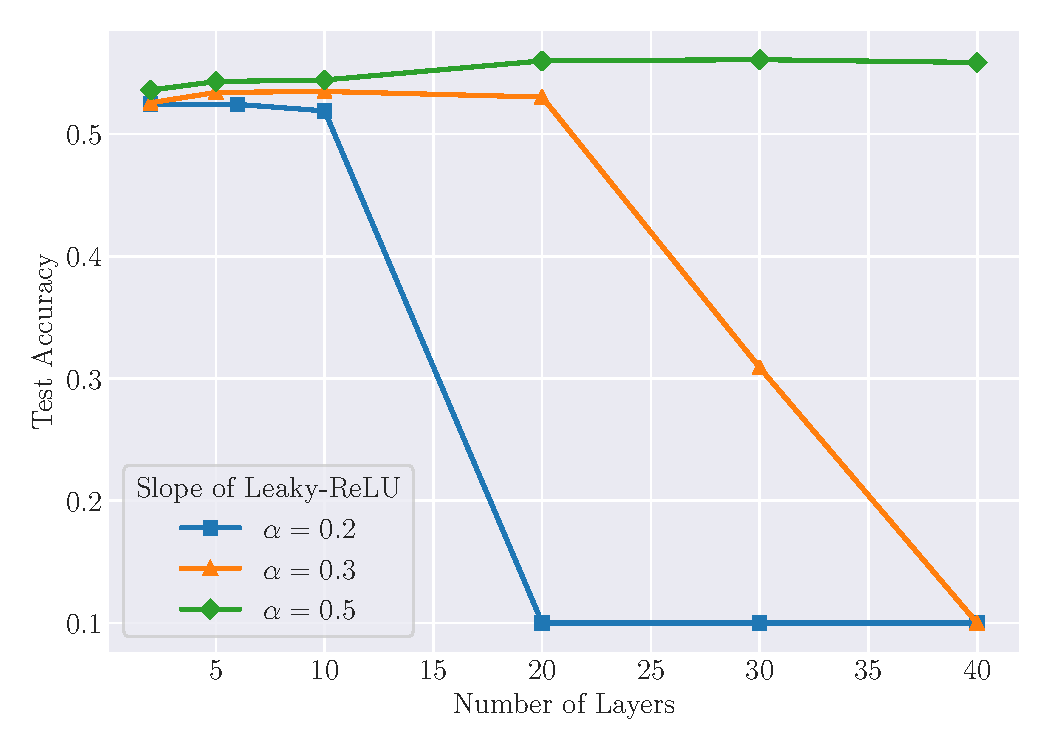
\includegraphics[width=\scalefigure\textwidth]{figures/main/ch4-diagonal_circulant/cifar10_leaky_relu.pdf}
  \caption{
    Impact of increasing the slope of a Leaky-ReLU in DCNNs.
    Deep DCNNs with a larger slope are easier to train.}
  \label{figure:ch4-cifar10_leaky_relu}
\end{figure}


We empirically found that the ReLU activations had an impact on the training of deep diagonal-circulant neural networks.
Indeed, the deeper the network, the more nonlinear it is, which makes convergence difficult.
In an experiment, we replace the ReLU activations with Leaky-ReLU activations (\cf \Cref{subsection:ch2-preliminaries_on_neural_networks}) and vary the slope of the Leaky-ReLU (a higher slope means an activation function that is closer to a linear function).
The results of this experiment are presented in~\Cref{figure:ch4-cifar10_leaky_relu}.

% In \Cref{figure:ch4-cifar10_leaky_relu}, we observe that reducing the nonlinearity of the networks can be used to train deeper networks.
In the experiment, we try different slopes for the Leaky-ReLU activation and train diagonal-circulant neural networks with different depth.
We can observe that a higher slope (making the network more linear) facilitates convergence, allowing us to train deeper networks.
This is an interesting result, since  we can use this technique to adjust the number of parameters in the network (increasing depth), without facing training difficulties.
We hence rely on this setting in the experimental section. 

\pagebreak

% Indeed, the more nonlinear activation a network 
%
% reducing the number of nonlinearities in the networks simplifies the training of deep neural networks.
%
% To support this claim, we conduct a series of experiments on various DCNNs with a varying number of ReLU activations (to reduce the number of nonlinearities, we replace some ReLU activations with the identity function).
%
% In a second experiment, 
%
% \todotext{update here}
% Replacing the ReLU activation by the identity function is equivalent to varying the number of factor in a layer.
% In \Cref{figure:ch4-cifar10_factor}, we compare diagonal-circulant neural networks with several values of $k$ which set the number of factors inside a layer as follows:
% \begin{equation}
%   \rho \left( \prod_{i=1}^{k} \Dmat^{(i)}\Cmat^{(i)} \xvec + \bvec \right)
% \end{equation}
% % ``ReLU(DC)'' means that we interleave ReLU activation functions between every diagonal-circulant matrix, whereas ReLU(DCDC) means we interleave a ReLU activation every other block etc.
% In both \Cref{figure:ch4-cifar10_factor,figure:ch4-cifar10_leaky_relu}, we observe that reducing the nonlinearity of the networks can be used to train deeper networks.
% This is an interesting result, since  we can use this technique to adjust the number of parameters in the network, without facing training difficulties.
% We obtain a maximum accuracy of 0.56 with one ReLU every three layers and leaky-ReLUs with a slope of 0.5.
% We hence rely on this setting in the experimental section. 
%
% \begin{figure}[htb]
%    \centering
%    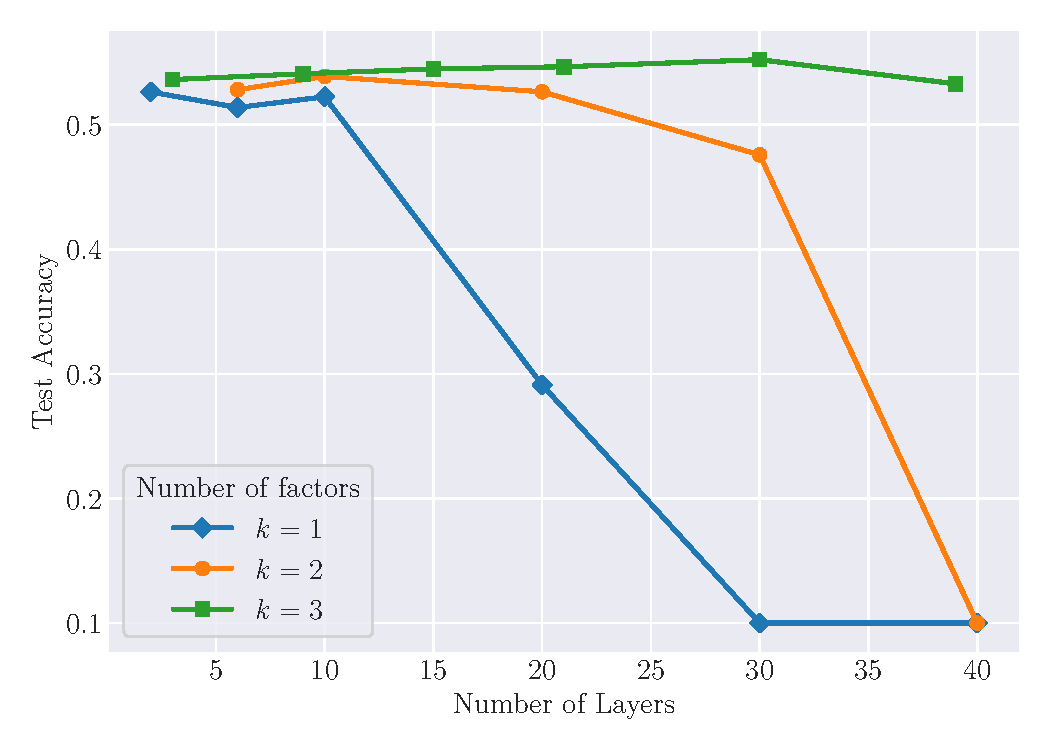
\includegraphics[width=\scalefigure\textwidth]{figures/main/ch4-diagonal_circulant/cifar10_factor.pdf}
%    \caption{
%       Impact of increasing the number of ReLU activations in a DCNN.
%       Deep DCNNs with fewer ReLUs are easier to train.}
%    \label{figure:ch4-cifar10_factor}
% \end{figure}


% \begin{figure}[ht]
%    \centering
%    \begin{subfigure}[b]{\textwidth}
%      \centering
%      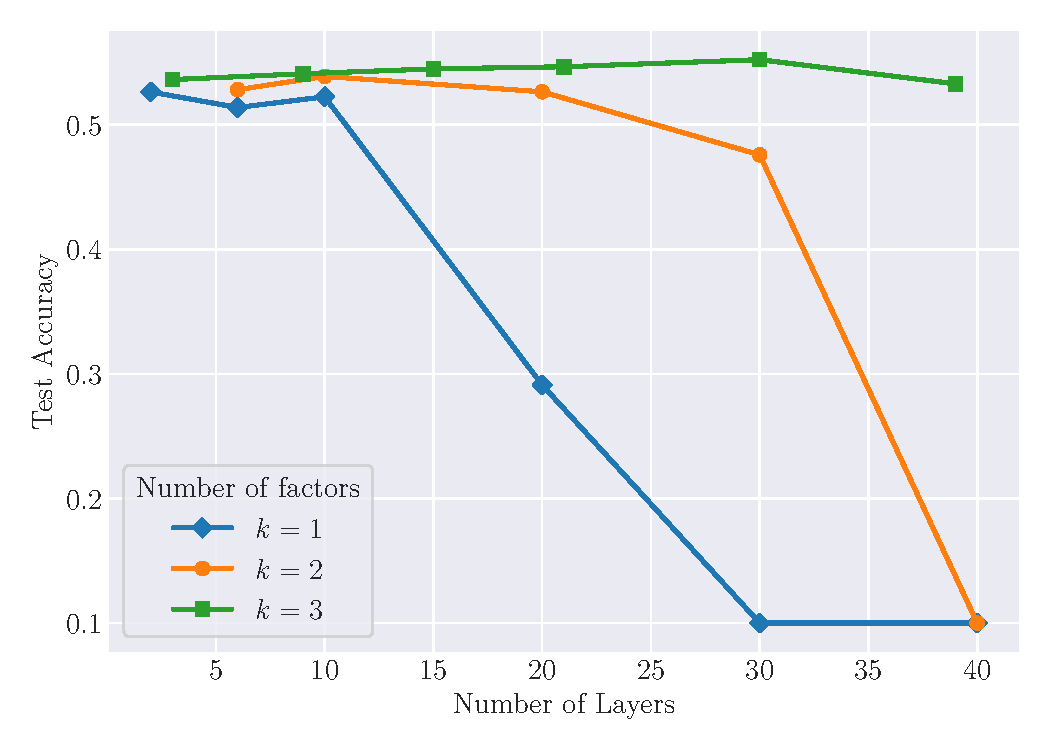
\includegraphics[width=\scalefigure\textwidth]{figures/main/ch4-diagonal_circulant/cifar10_factor.pdf}
%      \caption{
% 	Impact of increasing the number of ReLU activations in a DCNN.
% 	Deep DCNNs with fewer ReLUs are easier to train.}
%      \label{figure:ch4-cifar10_factor}
%    \end{subfigure}
%    \\[2cm]
%    \begin{subfigure}[b]{\textwidth}
%       \centering
%       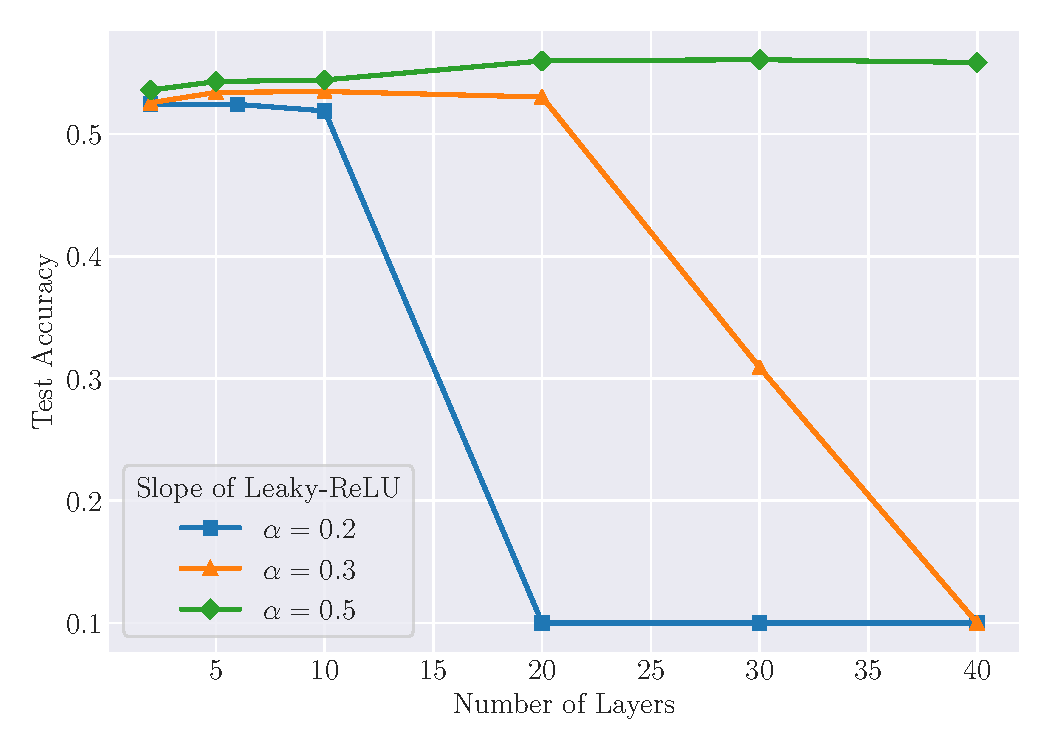
\includegraphics[width=\scalefigure\textwidth]{figures/main/ch4-diagonal_circulant/cifar10_leaky_relu.pdf}
%       \caption{
% 	Impact of increasing the slope of a Leaky-ReLU in DCNNs.
% 	Deep DCNNs with a larger slope are easier to train.}
%       \label{figure:ch4-cifar10_leaky_relu}
%    \end{subfigure}
%    \caption{xxx}
% \end{figure}



%%%%%%%%%%%%%%%%%%%%%%%%%%%%%%%%%%%%%%%%%%%%%%%%%%%%%%%%%%%%%%%%%%%%%%%%%%%%%%%
\section{Experiments}
\label{section:ch4-experiments}
%%%%%%%%%%%%%%%%%%%%%%%%%%%%%%%%%%%%%%%%%%%%%%%%%%%%%%%%%%%%%%%%%%%%%%%%%%%%%%%

This experimental section aims at answering the following questions:
\begin{enumerate}
    \itshape
    \item How do DCNNs compare to other approaches such as ACDC, LDR or other structured approaches?
    \item How do DCNNs compare to other compression based techniques?
    \item How do DCNNs perform in the context of large scale real-world machine learning applications?  
\end{enumerate}


%%%%%%%%%%%%%%%%%%%%%%%%%%%%%%%%%%%%%%%%%%%%%%%%%%%%%%%%%%%%%%%%%%%%%%%%%%%%%%%
\subsection{Comparison with other structured approaches}
\label{subsection:ch4-comparison_with_other_structured_approches}
%%%%%%%%%%%%%%%%%%%%%%%%%%%%%%%%%%%%%%%%%%%%%%%%%%%%%%%%%%%%%%%%%%%%%%%%%%%%%%%


% \begin{figure}
%    \centering
%    \begin{subfigure}[b]{0.75\textwidth}
%        \centering
%        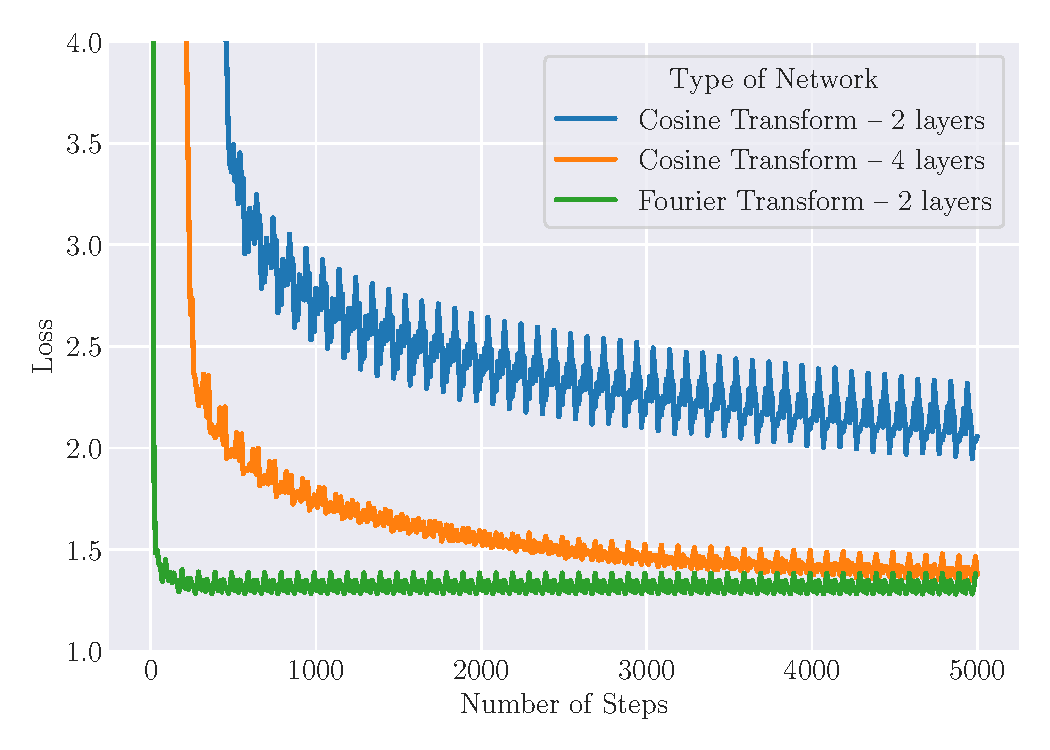
\includegraphics[width=\textwidth]{figures/main/ch4-diagonal_circulant/acdc_regression.pdf}
%        \caption{Evolution of the training loss on a regression task with synthetic data.}
%        \label{figure:ch4-acdc_regression}
%    \end{subfigure}
%    \\[2cm]
%    \begin{subfigure}[b]{0.75\textwidth}
%        \centering
%        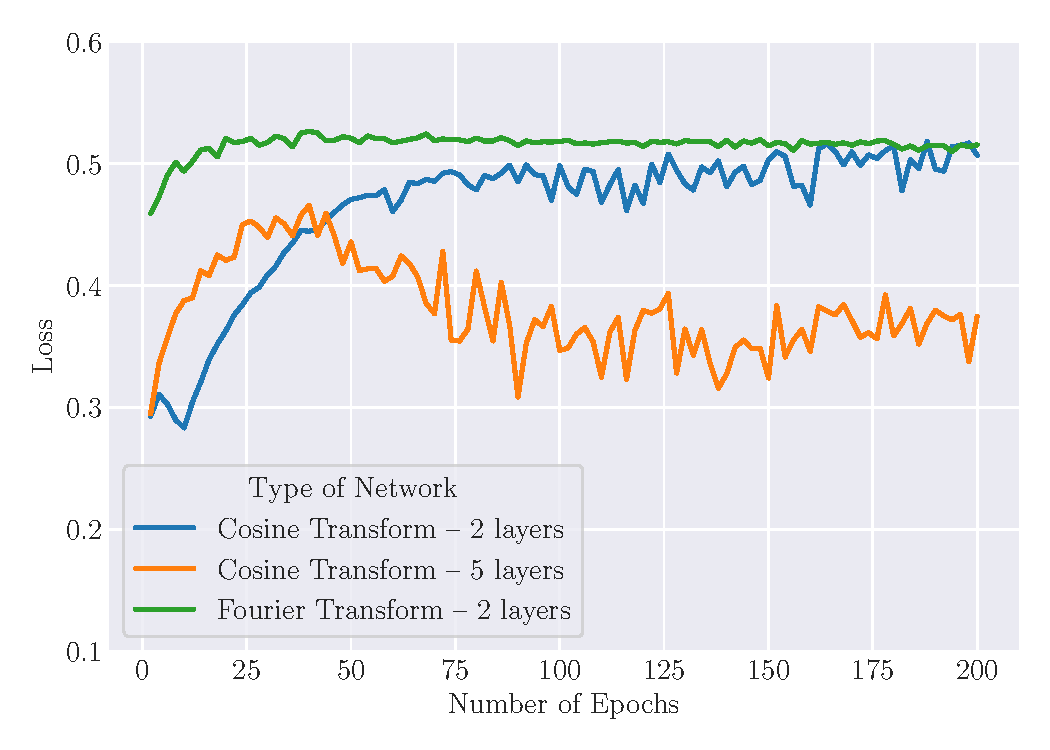
\includegraphics[width=\textwidth]{figures/main/ch4-diagonal_circulant/acdc_cifar10.pdf}
%        \caption{Test accuracy on the CIFAR-10 dataset.~\\ \phantom{.}}
%        \label{figure:ch4-acdc_cifar10}
%    \end{subfigure}
%    \caption{Comparison of DCNNs and \ACDC networks on two different tasks.}
% \end{figure}


\begin{figure}[ht]
   \centering
   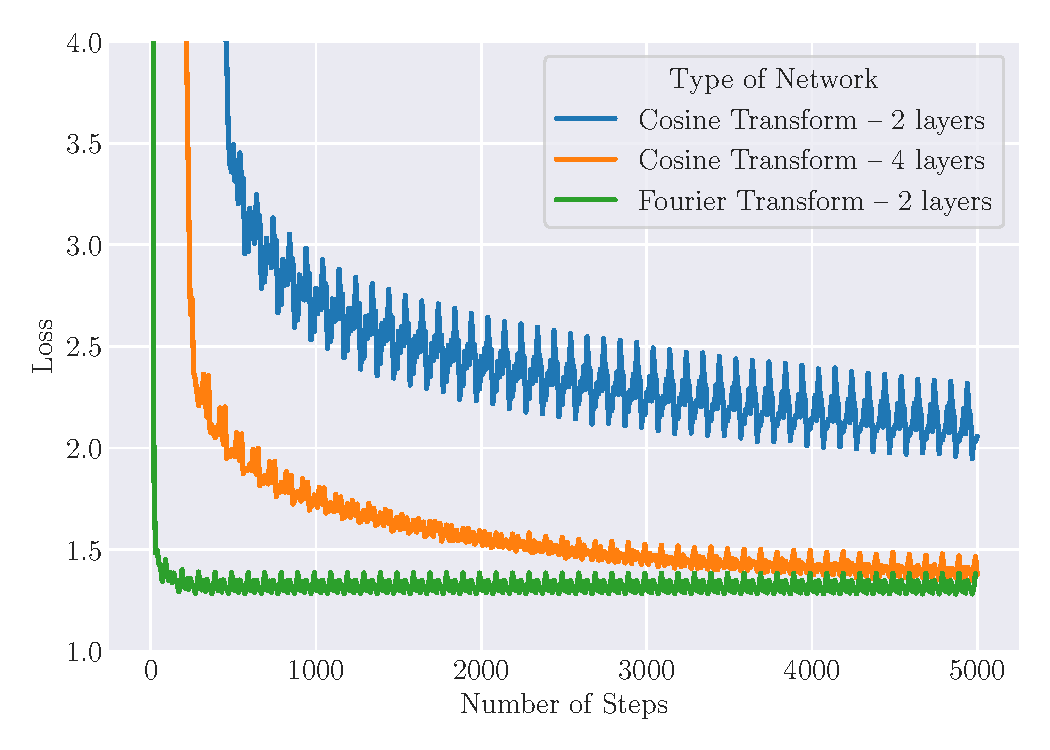
\includegraphics[width=\scalefigure\textwidth]{figures/main/ch4-diagonal_circulant/acdc_regression.pdf}
   \caption{Evolution of the training loss on a regression task with synthetic data.}
   \label{figure:ch4-acdc_regression}
\end{figure}

\begin{figure}[ht]
   \centering
   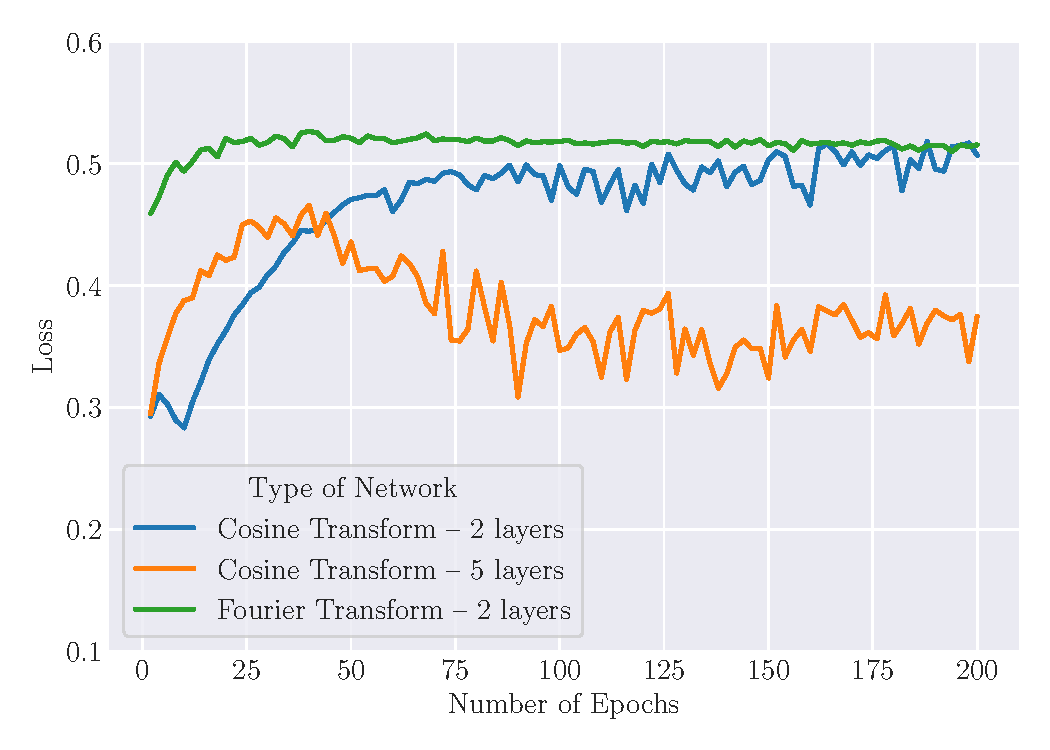
\includegraphics[width=\scalefigure\textwidth]{figures/main/ch4-diagonal_circulant/acdc_cifar10.pdf}
   \caption{Comparison of DCNNs and \ACDC networks on two different tasks. - Test accuracy on the CIFAR-10 dataset.}
   \label{figure:ch4-acdc_cifar10}
\end{figure}



%%%%%%%%%%%%%%%%%%%%%%%%%%%%%%%%%%%%%%%%%%%%%%%%%%%%%%%%%%%%%%%%%%%%%%%%%%%%%%%
\subsubsection{Comparison with \ACDC}
%%%%%%%%%%%%%%%%%%%%%%%%%%%%%%%%%%%%%%%%%%%%%%%%%%%%%%%%%%%%%%%%%%%%%%%%%%%%%%%

In \Cref{chapter:ch3-related_work}, we have discussed the differences between the \ACDC framework and our approach from a theoretical perspective.
In this section, we conduct experiments to compare the performance of DCNNs with neural networks based on \ACDC layers. 
We first reproduce the experimental setting from \citet{moczulski2016acdc}, and compare both approaches using only linear networks (\ie networks without any ReLU activations).
The synthetic dataset has been created in order to reproduce the experiment on the regression linear problem proposed by~\citet{moczulski2016acdc}.
We draw $\Xmat$ and $\Wmat$ from a uniform distribution between [-1, +1] and $\epsilon$ from a normal distribution with mean 0 and variance $0.01$.
The relationship between $\Xmat$ and $\Ymat$ is defined by $\Ymat = \Xmat\Wmat + \epsilon$. 
The results are presented in \Cref{figure:ch4-acdc_regression}.
In this simple setting, while both architectures demonstrate good performance, we can observe that DCNNs offer a better convergence rate.
In \Cref{figure:ch4-acdc_cifar10}, we compare neural networks with ReLU activations on CIFAR-10. 

We found that networks which are based only on \ACDC layers are difficult to train and offer poor accuracy on CIFAR-10 (we have tried different initialization schemes including the one from the original paper, and the one we introduce in this chapter).
\citet{moczulski2016acdc} manage to train a large VGG network  however these networks are generally highly redundant and the contribution of the structured layer is difficult to quantify. 
We also observe that adding a single dense layer improves the convergence rate of \ACDC in the linear case, which explains the good results of \citet{moczulski2016acdc}.
However, it is difficult to characterize the true contribution of the \ACDC layers when the network has a large number of expressive layers.

In contrast, deep DCNNs can be trained and offer good performance without additional dense layers (these results are in line with our experiments on the \yt dataset).
We can conclude that DCNNs are able to model complex relations at a low cost. 

% \begin{figure}
%    \centering
%    \begin{tikzpicture}[scale=0.8]
\begin{axis}[
    legend cell align={left},
    xlabel={\large \#weights (x1000) },
    ylabel={Test Accuracy},
    xmin=21, xmax=370,
    ymin=0.2, ymax=0.6,
    legend pos=south east,
    ymajorgrids=true,
    grid style=dashed,
	]
    \addplot[color=red, line width=0.25mm, dashed] table [y=accuracy, x=weights]
    {figures/main/ch4-diagonal_circulant/data/cifar10/type/dense.dat};
    \addplot[mark=triangle, color=blue, line width=0.4mm] table [y=accuracy, x=weights]
    {figures/main/ch4-diagonal_circulant/data/cifar10/type/circulant.dat};
    \addplot[mark=square, color=red, line width=0.4mm] table [y=accuracy, x=weights]
    {figures/main/ch4-diagonal_circulant/data/cifar10/type/diag_toeplitz.dat};
    \addplot[mark=o, color=gray, line width=0.4mm] table [y=accuracy, x=weights]
    {figures/main/ch4-diagonal_circulant/data/cifar10/type/toeplitz.dat};
    \addplot[mark=diamond, color=brown, line width=0.4mm] table [y=accuracy, x=weights]
    {figures/main/ch4-diagonal_circulant/data/cifar10/type/low_rank.dat};
    \legend{
      Dense (9M weights),
      DCNN,
      DTNN,
      Toeplitz network,
      Low Rank network, 
     }
\end{axis}
\end{tikzpicture}

%    \caption{Network size vs. Accuracy compared on Dense networks, DCNNs (our approach), DTNNs (our approach), neural networks based on Toeplitz matrices and neural networks based on Low Rank-based matrices. DCNNs outperforms alternatives structured approaches.}
%    \label{figure:ch4-cifar10_type}
% \end{figure}


\begin{figure}
   \centering
   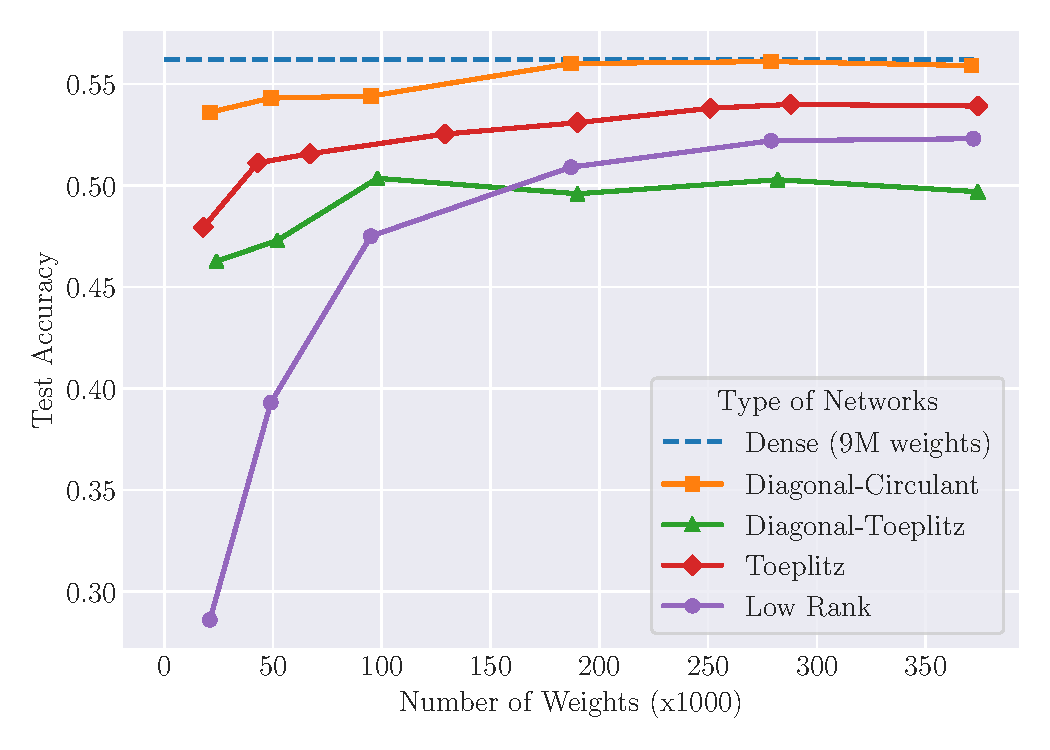
\includegraphics[width=\scalefigure\textwidth]{figures/main/ch4-diagonal_circulant/cifar10_type.pdf}
   \caption{Network size vs. Accuracy compared on Dense networks, DCNNs (our approach), DTNNs (our approach), neural networks based on Toeplitz matrices and neural networks based on Low Rank-based matrices. DCNNs outperforms alternatives structured approaches.}
   \label{figure:ch4-cifar10_type}
\end{figure}



\begin{figure}
   \centering
   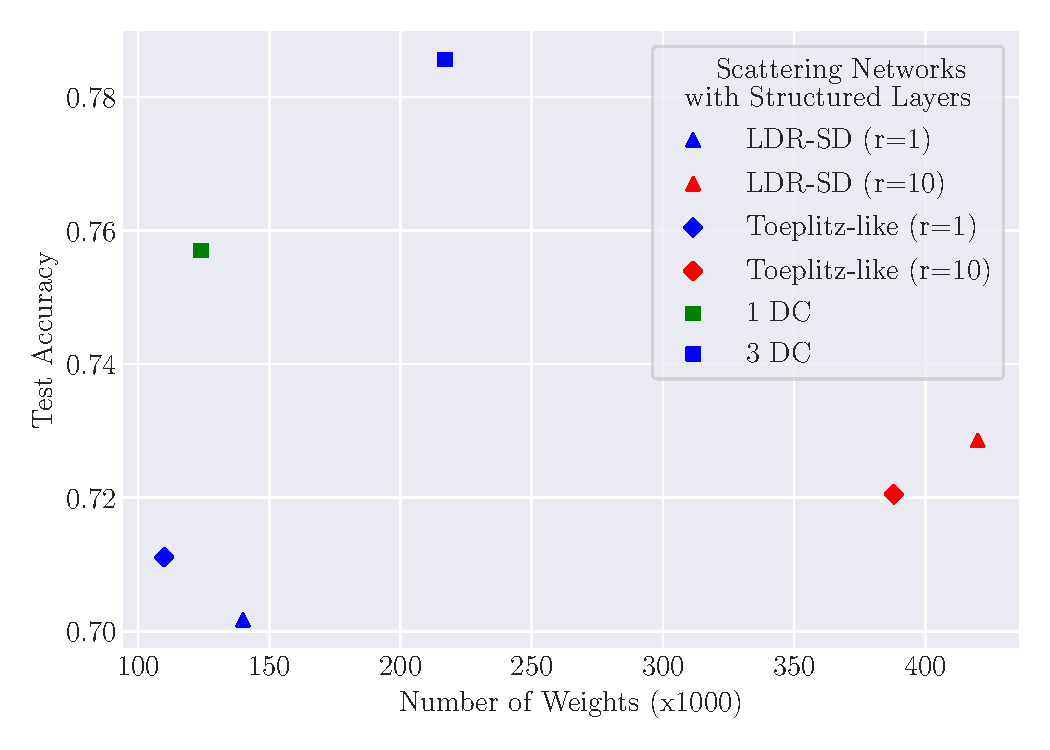
\includegraphics[width=\scalefigure\textwidth]{figures/main/ch4-diagonal_circulant/scatterplot.pdf}
   \caption{Accuracy of different structured architecture given the number of trainable parameters.}
   \label{figure:ch4-cifar10_with_channels_xp}
\end{figure}




%%%%%%%%%%%%%%%%%%%%%%%%%%%%%%%%%%%%%%%%%%%%%%%%%%%%%%%%%%%%%%%%%%%%%%%%%%%%%%%
\subsubsection{Comparison with Dense networks, Toeplitz networks and Low Rank networks.}
%%%%%%%%%%%%%%%%%%%%%%%%%%%%%%%%%%%%%%%%%%%%%%%%%%%%%%%%%%%%%%%%%%%%%%%%%%%%%%%

We now compare DCNNs with other state-of-the-art structured networks by measuring the accuracy on a flattened version of the CIFAR-10 dataset.
Our baseline is a dense feed-forward network with a fixed number of weights (9 million weights).
We compare with DCNNs and with DTNNs (see below), Toeplitz networks, and Low-Rank networks~\cite{yu2017compressing}.
We first consider Toeplitz networks which are stacked Toeplitz matrices interleaved with ReLU activations since Toeplitz matrices are closely related to circulant matrices.
However, Toeplitz networks have a different structure than DCNNs (they do not include diagonal matrices), therefore, we also experiment using DTNNs, a variant of DCNNs where all the circulant matrices have been replaced by Toeplitz matrices.
Finally we conduct experiments using networks based on low-rank matrices as they are also closely related to our work.
For each approach, we report the accuracy of several networks with a varying depth ranging from 1 to 40 (DCNNs, Toeplitz networks) and from 1 to 30 (from DTNNs).
For low-rank networks, we used a fixed depth network and increased the rank of each matrix from 7 to 40.
We also tried to increase the depth of low rank matrices, but we found that deep low-rank networks are difficult to train so we do not report the results here.
We compare all the networks based on the number of weights from 21K (0.2\% of the dense network) to 370K weights (4\% of the dense network) and we report the results in \Cref{figure:ch4-cifar10_type}. 
First we can see that the size of the networks correlates positively with their accuracy which demonstrated successful training in all cases.
We can also see that the DCNNs achieves the maximum accuracy of 56\% with 20 layers ($\sim$ 200K weights) which is as good as the dense networks with only 2\% of the number of weights.
Other approaches also offer good trade-offs but they are not able to reach the accuracy of a dense network.


%%%%%%%%%%%%%%%%%%%%%%%%%%%%%%%%%%%%%%%%%%%%%%%%%%%%%%%%%%%%%%%%%%%%%%%%%%%%%%%
\subsubsection{Comparison with LDR networks}
%%%%%%%%%%%%%%%%%%%%%%%%%%%%%%%%%%%%%%%%%%%%%%%%%%%%%%%%%%%%%%%%%%%%%%%%%%%%%%%

\begin{table}[htb]
  \centering
  \begin{tabular}{lcc}
    \toprule
    \textbf{Architectures} & \textbf{\#Parameters} & \textbf{Accuracy}  \\
    \midrule
    \textit{Dense} & \textit{9.4M}	 & \textit{0.562} \\
    \textbf{\textit{DCNN $(5\ layers)$}} & \textbf{49K}	& \textbf{0.543} \\
    \textbf{\textit{DCNN $(2\ layers)$}} & \textbf{21K} & \textbf{0.536} \\
    LDR--TD	$(r = 2)$	         & 64K	& 0.511 \\
    LDR--TD	$(r = 3)$	         & 70K	& 0.473 \\
    Toeplitz-like $(r=2)$	         & 46K	& 0.483 \\
    Toeplitz-like $(r =3)$	         & 52K  & 0.496 \\
    \bottomrule
    \end{tabular}
    \caption{LDR networks compared with DCNNs on a flattend version of CIFAR-10. DCNNs outperform all LDR configurations with fewer weights. Remark: the numbers may differ from the original experiments by~\citet{thomas2018learning} because we use the original dataset instead of a monochrome version.}
    \label{table:ch4-xp_ldr}
\end{table}

We now compare DCNNs with the LDR framework using the network configuration experimented in the original paper \cite{thomas2018learning}: a single LDR structured layer followed by a dense layer.
In the LDR framework, we can change the size of a network by adjusting the rank of the residual matrix, effectively capturing matrices with a structure that is close to a known structure but not exactly (in the LDR framework, Toeplitz matrices can be encoded with a residual matrix with rank=2, so a matrix that can be encoded with a residual of rank=3 can be seen as Toeplitz-like.).
The results are presented in \Cref{table:ch4-xp_ldr} and demonstrate that DCNNs outperforms all LDR networks both in terms in size and accuracy.


%%%%%%%%%%%%%%%%%%%%%%%%%%%%%%%%%%%%%%%%%%%%%%%%%%%%%%%%%%%%%%%%%%%%%%%%%%%%%%%
\subsection{Comparison with other compression based approaches}
\label{subsection:ch4-comparison_with_other_compression_based_approaches}
%%%%%%%%%%%%%%%%%%%%%%%%%%%%%%%%%%%%%%%%%%%%%%%%%%%%%%%%%%%%%%%%%%%%%%%%%%%%%%%


\begin{table}
  \centering
    \caption{Comparison with compression based approaches}
    \begin{tabular}{lcrc}
    \toprule
    \multicolumn{1}{c}{\textbf{Architecture}} & \multicolumn{1}{c}{\textbf{\#Params}} & \textbf{Error (\%)} \\
    \hline \\
    \textit{LeNet \cite{Lecun98gradient-basedlearning}} & \textit{4 257 674} & \textit{0.61} \\
    \multirow{2}[0]{*}{\textbf{DCNN}} & \textbf{25 620} & \textbf{1.74} \\
          & \textbf{31 764} & \textbf{1.60} \\
    \multirow{2}[0]{*}{HashNet \cite{chen2015compressing}} & 46 875 & 2.79 \\
          &  78 125 & 1.99 \\
    \multirow{2}[0]{*}{Dark Knowledge \cite{hinton2015distilling}} & 46 875 & 6.32 \\
          &  78 125 & 2.16 \\
    \bottomrule
    \end{tabular}%
  \label{tab:mnist}%
\end{table}%


We provide a comparison with other compression based approaches such as HashNet \cite{chen2015compressing}, Dark Knowledge \cite{hinton2015distilling} and Fast Food Transform (FF) \cite{yang2015deep}. 
\Cref{tab:mnist} shows the test error of DCNN against other known compression techniques on the MNIST datasets.
We can observe that DCNN outperforms HashNet \cite{chen2015compressing} and Dark Knowledge \cite{hinton2015distilling} with fewer number of parameters.
The architecture with Fast Food (FF) \cite{yang2015deep} achieves better performance but with convolutional layers and only $1$ Fast Food Layer as the last Softmax layer. 

%%%%%%%%%%%%%%%%%%%%%%%%%%%%%%%%%%%%%%%%%%%%%%%%%%%%%%%%%%%%%%%%%%%%%%%%%%%%%%%
\subsection{Large-scale video classification on the \yt dataset}
\label{subsection:ch4-large_scale_video_classification}
%%%%%%%%%%%%%%%%%%%%%%%%%%%%%%%%%%%%%%%%%%%%%%%%%%%%%%%%%%%%%%%%%%%%%%%%%%%%%%%

To understand the performance of deep DCNNs on large scale applications, we conducted experiments on the \yt video classification with 3.8 training examples introduced by~\citet{abu2016youtube}.
Notice that we favour this experiment over ImageNet applications because modern image classification architectures involve a large number of convolutional layers, and compressing convolutional layers is out of our scope. 
Also, as mentioned earlier, testing the performance of DCNN architectures mixed with a large number of expressive layers makes little sense.
The \yt includes two datasets describing 8 million labeled videos.
Both datasets contain audio and video features for each video.
In the first dataset (\emph{aggregated}) all audio and video features have been aggregated every 300 frames.
The second dataset (\emph{full}) contains the descriptors for all the frames.
To compare the models we use the GAP metric (Global Average Precision) proposed by~\citet{abu2016youtube}.
On the simpler \emph{aggregated} dataset we compared off-the-shelf DCNNs with a dense baseline with 5.7M weights.
On the full dataset, we designed three new compact architectures based on the state-of-the-art architecture introduced by~\citet{abu2016youtube}. 

\paragraph{Experiments on the aggregated dataset with DCNNs}
We compared DCNNs with a dense baseline with 5.7 millions weights.
The goal of this experiment is to discover a good trade-off between depth and model accuracy.
To compare the models we use the GAP metric (Global Average Precision) following the experimental protocol in~\cite{abu2016youtube}, to compare our experiments. 

\Cref{table:youtube_agg_xp} shows the results of our experiments on the \emph{aggregated} \yt dataset in terms of number of weights, compression rate and GAP.
We can see that the compression ratio offered by the circulant architectures is high.
This comes at the cost of a little decrease of GAP measure.
The 32 layers DCNN is 46 times smaller than the original model in terms of number of parameters while having a close performance. 


\begin{table}
  \centering
  \caption{This table shows the GAP score for the \yt dataset with DCNNs. We can see a large increase in the score with deeper networks.}
  \begin{tabular}{lccc}
    \toprule
    \textbf{Architecture} & \textbf{\#Weights} &
    \textbf{GAP@20} \\
    \hline \\
    \textit{original} & \textit{5.7M} & \textit{0.773} \\
    4 DC & 25 410  (\textit{\textbf{0.44}}) & 0.599   \\
    32 DC  & 122 178 \textit{(2.11)} & 0.685   \\
    4 DC + 1 FC & 4.46M \textit{(77)} & \textbf{0.747} \\
  \hline
  \end{tabular}
  \label{table:youtube_agg_xp}
\end{table}

\begin{table}
  \centering
  \caption{This table shows the GAP score for the \yt dataset with different layer represented with our DC decomposition.}
  \begin{tabular}{lccc}
  \toprule
  \textbf{Architecture} & \textbf{\#Weights} & \textbf{GAP@20} \\
  \hline \\
  \textit{original} & \textit{45M} & \textit{0.846} \\
  DBoF with DC   & 36M (\textit{80}) & 0.838 \\
  FC with DC    & 41M (\textit{91}) & \textbf{0.845} \\
  MoE with DC   & 12M (\textit{\textbf{26}}) & 0.805 \\
  \hline
  \end{tabular}
  \label{table:youtube_full_xp}
\end{table}

\paragraph{Experiments with DCNNs Deep Bag-of-Frames Architecture:}
The Deep Bag-of-Frames architecture can be decomposed into three blocks of layers, as illustrated in \Cref{figure:ch4-archi_youtube}.
The first block of layers, composed of the Deep Bag-of-Frames embedding (DBoF), is meant to model an embedding of these frames in order to make a simple representation of each video.
A second block of fully connected layers (FC) reduces the dimensionality of the output of the embedding and merges the resulting output with a concatenation operation.
Finally, the classification block uses a combination of Mixtures-of-Experts (MoE)~\cite{jordan1993hierarchical,abu2016youtube} and Context Gating~\cite{miech2017learnable} to calculate the final class probabilities.
\Cref{table:youtube_full_xp} shows the results in terms of number of weights, size of the model (MB) and GAP on the full dataset, replacing the DBoF block reduces the size of the network without impacting the accuracy.
We obtain the best compression ratio by replacing the MoE block with DCNNs (26\%) of the size of the original dataset with a GAP score of 0.805 (95\% of the score obtained with the original architecture).
We conclude that DCNN are both theoretically sound and of practical interest in real, large scale applications.

\begin{figure}[htb]
  \centering
  \tikzset{%
  >={Latex[width=2mm,length=2mm]},
  % Specifications for style of nodes:
            base/.style = {rectangle, draw=black, text centered, font=\sffamily},
             box/.style = {base, rounded corners, text depth=3cm, minimum height=4cm, minimum width=3cm},
     transparent/.style = {rectangle, draw=black},
       circulant/.style = {base, fill=yellow!30},
       embedding/.style = {base, fill=blue!30, minimum width=2.5cm, minimum height=1cm},
           other/.style = {base, fill=white!30,  minimum width=2cm, minimum height=1cm},
              fc/.style = {base, fill=orange!30, minimum width=1.5cm, minimum height=1cm},
          gating/.style = {base, fill=green!30, minimum width=2cm, text width=2cm, minimum height=1cm},
             moe/.style = {base, fill=purple!30, minimum width=1.5cm, minimum height=1cm},
}

\begin{tikzpicture}[every node/.style={fill=white, font=\sffamily}, align=center]

  \draw (0.0, +2.)  node [other, draw=none] {\textbf{Embedding}};
  \draw (+3.7, +2.)  node [other, draw=none] {\textbf{Dim Reduction}};
  \draw (+8.0, +2.)  node [other, draw=none] {\textbf{Classification}};

  \draw (0, +0.8)  node [embedding] {Video};
  \draw (0, -0.8)  node [embedding] {Audio};

  \draw (+2.5, +0.8)  node (fc) [fc] {FC};
  \draw (+2.5, -0.8)  node (fc) [fc] {FC};

  \draw (+4.75, 0)  node (fc) [other] {concat};
  \draw (+7.0, 0)  node (moe) [moe] {MoE};
  \draw (+9.25, 0)  node (gating2) [gating] {Context Gating};
 
  \draw (+1.5, +2) [dashed] -- (+1.5, -1.7);
  \draw (+6, +2) [dashed] -- (+6, -1.7);
  
\end{tikzpicture}

  \caption{This figure shows the state-of-the-art neural network architecture, initially proposed by~\citet{abu2016youtube} and later improved by~\citet{miech2017learnable}, used in our experiment.}
  \label{figure:ch4-archi_youtube}
\end{figure}

\paragraph{Architectures \& Hyper-Parameters:} 
For the first set of our experiments (\emph{experiments on CIFAR-10}), we train all networks for 200 epochs, a batch size of 200, Leaky ReLU activation with a different slope.
We minimize the Cross Entropy Loss with Adam optimizer and use a piecewise constant learning rate of $5 \times 10^{-5}$, $2.5\times10^{-5}$, $5\times10^{-6}$ and $1\times10^{-6}$ after respectively 40K, 60K and 80K steps.
For the \yt dataset experiments, we built a neural network based on state-of-the-art architecture initially proposed by~\citet{abu2016youtube} and later improved by~\citet{miech2017learnable}.
Remark that no convolution layer is involved in this application since the input vectors are embeddings of video frames processed using state-of-the-art convolutional neural networks trained on ImageNet.
We trained our models with the CrossEntropy loss and used Adam optimizer with a 0.0002 learning rate and a 0.8 exponential decay every 4 million examples.
All fully connected layers are composed of 512 units.
DBoF, NetVLAD and NetFV are respectively 8192, 64 and 64 of cluster size for video frames and 4096, 32, 32 for audio frames.
We used 4 mixtures for the MoE Layer.
We used all the available 300 frames for the DBoF embedding.
In order to stabilize and accelerate the training, we used batch normalization before each non linear activation and gradient clipping. 


%%%%%%%%%%%%%%%%%%%%%%%%%%%%%%%%%%%%%%%%%%%%%%%%%%%%%%%%%%%%%%%%%%%%%%%%%%%%%%%
\subsection{Exploiting Image Features}
%%%%%%%%%%%%%%%%%%%%%%%%%%%%%%%%%%%%%%%%%%%%%%%%%%%%%%%%%%%%%%%%%%%%%%%%%%%%%%%

\begin{table}[htb]
  \centering
  \begin{tabular}{lcc}
    \toprule
    \textbf{Architectures} & \textbf{\#Parameters} & \textbf{Accuracy}  \\
    \midrule
    \textbf{DC $(1\ layers)$} & \textbf{124K} & \textbf{0.757} \\
    \textbf{DC $(3\ layers)$} & \textbf{217K} & \textbf{0.785} \\
    % \textbf{Ensemble x5 DC $(3\ layers)$} &  \textbf{1.08M} & \textbf{0.811} \\
    LDR-SD $(r=1)$ & 140K & 0.701 \\
    LDR-SD $(r=10)$ & 420K & 0.728 \\
    Toeplitz-like $(r=1)$ & 110K & 0.711 \\
    Toeplitz-like $(r=10)$ & 388K & 0.720 \\
    \bottomrule
    \end{tabular}
    \caption{Two depths scattering on CIFAR-10 followed by LDR or DC layer. Networks with DC layers outperform all LDR configurations with fewer weights.}
    \label{table:ch4-xp_ldr_scattering}
\end{table}




Dense layers and DCNNs are not designed to capture task-specific features such as the translation invariance inherently useful in image classification.
We can further improve the accuracy of such general purpose architectures on image classification without dramatically increasing the number of trained parameters by stacking them on top of fixed (ie non-trained) transforms such as the scattering transform \cite{mallat2010recursive}.
In this section we compare the accuracy of various structured networks, enhanced with the scattering transform, on an image classification task, and run comparative experiments on CIFAR-10. 

Our test architecture consists of 2 depth scattering on the RGB images followed by a batch norm and LDR or DC layer.
To vary the number of parameters of Scattering+LDR architecture, we increase the rank of the matrix (stacking several LDR matrices quickly exhausted the memory).
The \Cref{figure:ch4-cifar10_with_channels_xp} and \Cref{table:ch4-xp_ldr_scattering} shows the accuracy of these architectures given the number of trainable parameters.

First, we can see that the DCNN architecture very much benefits from the scattering transform and is able to reach a competitive accuracy over 78\%.
We can also see that scattering followed by a DC layer systematically outperforms scattering + LDR or scattering + Toeplitz-like with less parameters. 





%%%%%%%%%%%%%%%%%%%%%%%%%%%%%%%%%%%%%%%%%%%%%%%%%%%%%%%%%%%%%%%%%%%%%%%%%%%%%%%
\section{Conclusion}
\label{section:ch4-discussion}
%%%%%%%%%%%%%%%%%%%%%%%%%%%%%%%%%%%%%%%%%%%%%%%%%%%%%%%%%%%%%%%%%%%%%%%%%%%%%%%

% \todotext{review this conclusion}
% \todotext{we need to open on the next chapter}

This chapter deals with the training of diagonal circulant neural networks.
To the best of our knowledge, training such networks with a large number of layers had not been done before.
We also endowed this kind of models with theoretical guarantees, hence enriching and refining previous theoretical work from the literature.
More importantly, we showed that DCNNs outperform their competing structured alternatives, including the very recent general approach based on LDR networks.
Our results suggest that stacking diagonal circulant layers with non linearities improves the convergence rate and the final accuracy of the network.
Formally proving these statements constitutes the future directions of this work.
We would like to generalize the good results of DCNNs to convolutional neural networks.
We also believe that circulant matrices deserve a particular attention in deep learning because of their strong ties with convolutions: a circulant matrix operator is equivalent to the convolution operator with circular paddings.
This fact makes any contribution to the area of circulant matrices particularly relevant to the field of deep learning with impacts beyond the problem of designing compact models.
As future work, we would like to generalize our results to deep convolutional neural networks. 

